%% Manuscript prepared with the ACM "acmart" class (acmart-primary, v2.20), following samples/acmsmall.tex.
%% For submission and review:  \documentclass[manuscript, screen, review]{acmart}
%% For camera-ready:            \documentclass[acmsmall]{acmart}
\documentclass[manuscript, screen, review]{acmart}

%% \BibTeX command to typeset BibTeX logo in the docs
\AtBeginDocument{%
  \providecommand\BibTeX{{%
    Bib\TeX}}}

%% Rights management information. Replace with the values provided when
%% completing the rights form.
\setcopyright{acmlicensed}
\copyrightyear{2026}
\acmYear{2026}
\acmDOI{XXXXXXX.XXXXXXX}

%% Journal information. acmart v2.20 has no code for ACM Collective
%% Intelligence; set \acmJournal to the code supplied by the journal's
%% author instructions (the sample uses JACM as a placeholder).
%% \acmJournal{JACM}
\acmVolume{1}
\acmNumber{1}
\acmArticle{1}
\acmMonth{10}

%% Submission ID (if provided by the journal).
%%\acmSubmissionID{}

\usepackage{amsmath}
\usepackage{algorithm}
\usepackage{algorithmic}
\usepackage{array}
\usepackage{makecell}
\usepackage{pifont}
\usepackage{booktabs}
\usepackage{multirow}
\usepackage{graphicx}
\usepackage{tikz}
\usetikzlibrary{arrows.meta,positioning,fit,shapes.geometric,calc}

\newcommand{\cmark}{\ding{51}}
\newcommand{\xmark}{\ding{55}}
% Shared TikZ styles for the framework diagrams (original vector drawings)
\tikzset{
  agent/.style={draw, rounded corners=2pt, fill=blue!6, align=center, font=\footnotesize, minimum height=8mm, inner sep=3pt},
  wm/.style={draw, rounded corners=2pt, fill=orange!10, align=center, font=\footnotesize, inner sep=4pt},
  op/.style={draw, fill=white, align=center, font=\scriptsize, inner sep=2.5pt, rounded corners=1pt},
  gate/.style={draw, diamond, aspect=2.2, fill=green!8, align=center, font=\scriptsize, inner sep=1pt},
  st/.style={draw, circle, fill=white, font=\scriptsize, inner sep=1.2pt, minimum size=6.5mm},
  flow/.style={-{Latex[length=1.8mm]}, semithick},
  fb/.style={-{Latex[length=1.8mm]}, semithick, dashed, red!65!black},
  lbl/.style={font=\scriptsize, align=center, fill=white, inner sep=1pt},
  panel/.style={draw=gray!60, rounded corners=3pt, inner sep=6pt},
  ttl/.style={font=\footnotesize\bfseries},
}

\emergencystretch=2em
\makeatletter
\newcommand{\tabinput}[1]{\@@input #1 }
\makeatother

%%
%% end of the preamble, start of the body of the document source.
\begin{document}

% earlier working title: When LLM Reviewers Agree Too Much: Correlated Errors and Acceptance Mechanisms in Multi-Agent Reasoning
\title{Independence Before Coordination: Why LLM Collectives Fail to Correct Shared Errors}

\author{Yu Wang}
\email{ywang4704@gatech.edu}
\orcid{0000-0000-0000-0000}
\affiliation{%
  \institution{College of Computing, Georgia Institute of Technology}
  \city{Atlanta}
  \state{Georgia}
  \country{USA}
}

\author{Vijay K. Madisetti}
\email{vkm@gatech.edu}
\orcid{0000-0000-0000-0000}
\affiliation{%
  \institution{School of Cybersecurity and Privacy, Georgia Institute of Technology}
  \city{Atlanta}
  \state{Georgia}
  \country{USA}
}

\renewcommand{\shortauthors}{Wang and Madisetti}

\begin{abstract}
Multi-agent systems built on large language models (LLMs) are collectives: an author agent proposes an answer, reviewer agents critique it, and a meta-reviewer decides.
The classical conditions under which a collective outperforms its members---independent judgments and diverse errors---are rarely checked in such systems.
We check them in a controlled study of a reviewer-style pipeline on eight reasoning benchmarks with four backbone LLMs, evaluating every configuration on identical questions in two independent runs with paired tests, and logging the author's first draft so that the effect of the collective can be measured within each run.
The collective almost never corrects its members: the meta-reviewer accepts 80--97\% of incorrect drafts in the first round, the four-agent process raises accuracy over the author's draft by 0.3--1.9 points, and the most capable backbone is the one whose reviewers agree most.
We then test mechanisms that take the acceptance decision away from the agents.
A lightweight world model that stores every candidate as an explicit state, validates transitions, estimates a trajectory risk from the reviews, and gates acceptance centrally blocks most incorrect drafts, but also most correct ones; the author repairs a blocked error in only 7--23\% of cases, and the net gain over the draft (0.0--1.8 points) is no larger than that of the ungated pipeline, at 1.7--4.3 times the cost.
A gain of 4.3 points observed on one backbone in the first run was not reproduced in the second; the run-to-run variation of a fixed configuration on fixed questions (up to 4 points) is as large as any difference between configurations.
A decentralized variant that keeps local state replicas but leaves acceptance to the agents is indistinguishable from the message-based pipeline, and a coordination-uncertainty index computed from reviewer disagreement does not predict which variant is preferable.
An exploratory gate based on agreement among reviewer answers is precise and cheap but low in recall, because in 80\% of the cases where the author is wrong both reviewers reproduce the same wrong answer; hiding the draft from the reviewers reduces this rate to 48--61\% in two runs, whereas giving the reviewers a different backbone while still showing them the draft does not change it. Crossing blind reviewers with the world-model gate shows that an LLM meta-reviewer who sees the draft overrules the independent reviewers and reintroduces the dependence, while the gate's risk estimate becomes more selective once its evidence is independent.
Across all methods, including debate-style baselines, collaboration improves on a single chain-of-thought call by at most about two points.
Taken together, homogeneous LLM collectives exhibit highly correlated judgments and limited error correction, which undermines a key condition for collective intelligence; decomposing their behaviour into detection, challenge, and repair shows that the dominant loss occurs before reconsideration begins, and that in this setting the binding constraint is the independence of the members---in particular their exposure to the candidate answer---rather than the representation of shared state or the communication topology. Collective intelligence in such systems requires not merely multiple agents but sufficiently independent evidence generation together with selective external oversight. We propose the agreement and repair statistics introduced here as standard diagnostics for multi-agent reasoning systems.
\end{abstract}

\begin{CCSXML}
<ccs2012>
<concept><concept_id>10010147.10010178.10010199</concept_id><concept_desc>Computing methodologies~Multi-agent systems</concept_desc><concept_significance>500</concept_significance></concept>
<concept><concept_id>10010147.10010178.10010179</concept_id><concept_desc>Computing methodologies~Natural language processing</concept_desc><concept_significance>300</concept_significance></concept>
</ccs2012>
\end{CCSXML}
\ccsdesc[500]{Computing methodologies~Multi-agent systems}
\ccsdesc[300]{Computing methodologies~Natural language processing}

\keywords{collective intelligence, large language models, multi-agent reasoning, correlated errors, acceptance mechanisms, world models}

\received{XX Month 2026}
\received[revised]{XX Month 2026}
\received[accepted]{XX Month 2026}

\maketitle

\section{Introduction}

A collective is only as intelligent as the independence of its members allows.
Condorcet's jury theorem, the wisdom-of-crowds literature, and the theory of informational cascades all say the same thing in different vocabularies: aggregating the judgments of several agents helps when their errors are diverse and independent, and stops helping---or hurts---when the agents see and follow one another~\cite{ladha1992condorcet,surowiecki2004wisdom,lorenz2011social,bikhchandani1992cascades}.

Multi-agent systems built on large language models (LLMs) are collectives of a particular kind. In the reviewer-style pipelines that have become common~\cite{du2024improving,liang2024mad,chen2024reconcile,wang2025mars}, an \emph{author} agent proposes an answer, \emph{reviewer} agents critique it, and a \emph{meta-reviewer} decides whether to accept it or send it back. The members of this collective are typically instances of the same model, and each reads the output of the others before judging. Both properties threaten the independence condition. Yet the question of whether such a collective actually corrects its members is seldom asked; evaluations report final accuracy, which conflates what the author would have answered alone with what the collective added.

This paper asks that question directly, and then asks what can be done about the answer.
We instrument a reviewer-style pipeline so that the author's first draft is logged in every run, which makes the contribution of the collective measurable \emph{within} a run as the change from draft accuracy to final accuracy, together with the rates at which wrong answers are caught and right answers are lost.
We evaluate every configuration on identical questions from eight reasoning benchmarks with four backbone LLMs, in two independent runs, with paired statistical tests.

The first result is that the collective rarely acts. Without an external acceptance mechanism, the meta-reviewer accepts 80--97\% of incorrect drafts in the first round; the four-agent process raises accuracy over the author's draft by 0.3--1.9 points; and the most capable backbone is the one whose reviewers agree with the author most (on 796 runs it changes four answers).

We then study mechanisms that take the acceptance decision away from the agents, in the spirit of world models in reinforcement learning~\cite{ha2018recurrent,hafner2020dream}: a symbolic state store that records every candidate solution as an explicit state, validates transitions, estimates a trajectory-level risk from the reviews, and, in its \emph{centralized} form, gates acceptance independently of any agent's verdict (Fig.~\ref{fig:concept}). A \emph{peer-to-peer} form keeps local state replicas and leaves acceptance to the agents. We also define a Coordination Uncertainty Index (CUI) from reviewer disagreement and test whether it predicts which form is preferable.

The second result is that an external gate does act, but with little discrimination and at a price: it blocks most incorrect drafts but also most correct ones, a blocked error is repaired by the author in only 7--23\% of cases, and its net effect over the draft (0.0--1.8 points) is no larger than that of the ungated pipeline, at up to 4.3 times the token cost. A gain of 4.3 points on one backbone in the first run disappeared in the second; the run-to-run variation of one configuration on fixed questions is as large as any difference between configurations. The peer-to-peer form has no measurable effect, and the CUI does not predict which form to use.

The third result points to what matters. An ablation shows that the behavioural effect of the gate---fewer incorrect drafts accepted at first sight---is obtained at a third of the cost by merely showing the risk signal to the deciding agent, and an exploratory gate that accepts a draft only when independently derived reviewer answers agree with it is precise and cheap---but it catches only 20\% of errors, because in 80\% of the cases where the author is wrong both reviewers reproduce the same wrong answer. The errors of the collective are correlated, exactly as the classical theory predicts for members who share a model and read each other's output. A direct test confirms the mechanism: reviewers that never see the draft reproduce the author's error substantially less often (48--61\% against 80\% in two runs), while reviewers from a different backbone that do see it reproduce it just as often. Crossing blind reviewers with the gate shows where oversight must sit: a draft-exposed LLM judge at the aggregation stage overrules the independent reviewers, whereas a rule that aggregates their answers and returns their solutions to the author does not.

We organize the study around five questions:
\begin{itemize}
    \item \textbf{RQ1} Do reviewer-style LLM collectives actually correct the errors of their members?
    \item \textbf{RQ2} If not, why: do the reviewers reproduce the author's errors?
    \item \textbf{RQ3} Is the correlation due to model homogeneity or to information dependence on the candidate answer?
    \item \textbf{RQ4} Can external oversight---a world-model gate that does not rely on the agents' agreement---help?
    \item \textbf{RQ5} Which part of such a world model matters, and can oversight and independence be combined?
\end{itemize}

Our contributions are three.
\begin{itemize}
    \item \textbf{Measurement.} A within-run diagnostic for multi-agent reasoning that follows every question from the author's first draft through reviewer agreement, interception, revision, and repair (Fig.~\ref{fig:flow}), instead of reporting final accuracy alone; together with a measurement of run-to-run variation that bounds what single-run comparisons can show (Section~\ref{sec:agreement}).
    \item \textbf{Empirical finding.} Across four backbone LLMs, 1{,}592 paired questions, and two independent runs, homogeneous reviewer-style collectives show very high agreement with incorrect drafts, so that multi-agent interaction rarely changes the answer, and the strongest backbone is the one that changes it least (Section~\ref{sec:agreement}).
    \item \textbf{Mechanism and intervention.} Interventions that force reconsideration---a centralized world-model gate, a risk-only variant, and gates based on answer agreement---raise the number of challenged drafts but are limited by weak discrimination and, above all, by correlated errors: when the author is wrong, independent reviewers usually produce the same wrong answer. Hiding the candidate answer from the reviewers reduces the reproduction of errors from 80\% to 48--61\%; changing the reviewers' backbone does not. Two hypotheses of our own earlier work, that decentralized coordination helps on uncertain tasks and that an uncertainty index predicts the preferable topology, are not supported; changing the topology does not create independence either (Sections~\ref{sec:mechanisms}--\ref{sec:topology}).
\end{itemize}
The state-centric framework of Section~\ref{sec:method} is the instrument with which these interventions are implemented and measured; we do not claim it as a contribution in itself.

\begin{figure*}[!t]
    \centering
    \resizebox{\textwidth}{!}{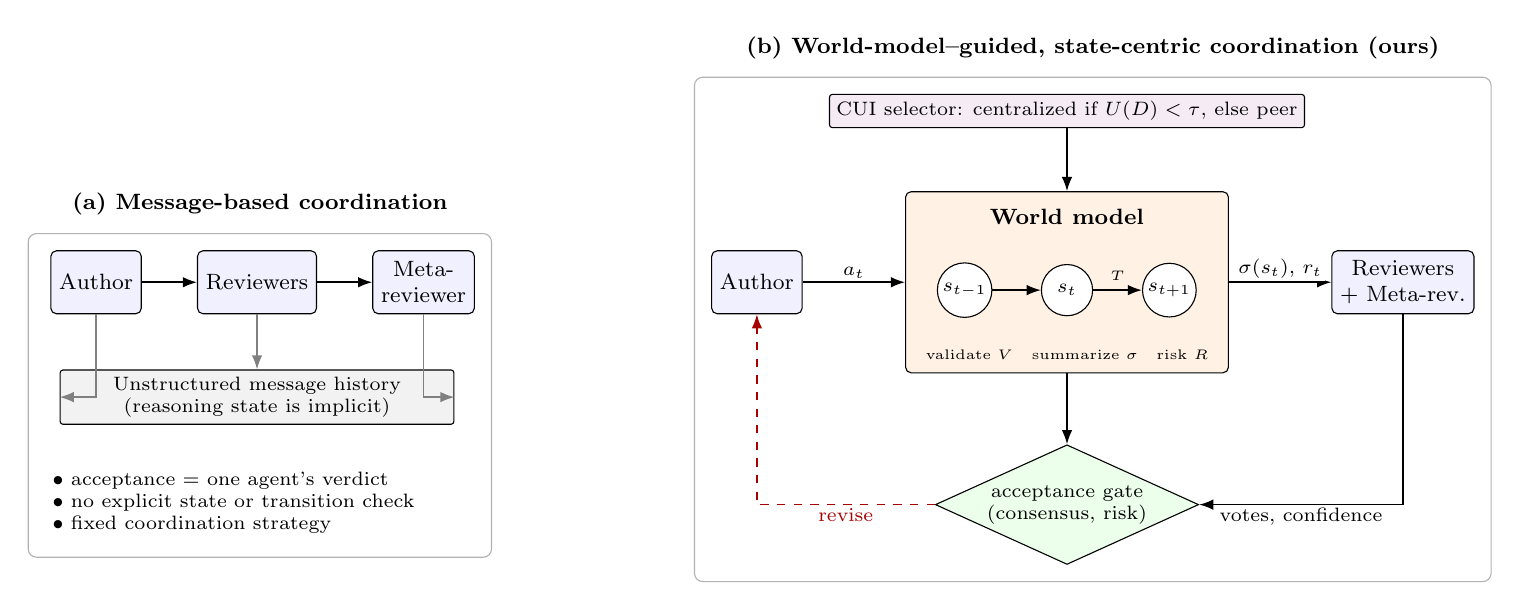
\begin{tikzpicture}[node distance=6mm and 7mm]
% ---------------- (a) message-based ----------------
\node[agent] (a1) {Author};
\node[agent, right=of a1] (r1) {Reviewers};
\node[agent, right=of r1] (m1) {Meta-\\reviewer};
\draw[flow] (a1) -- (r1);
\draw[flow] (r1) -- (m1);
\node[op, below=7mm of r1, minimum width=50mm, fill=gray!10] (hist) {Unstructured message history\\(reasoning state is implicit)};
\draw[flow, gray] (a1) |- (hist.west);
\draw[flow, gray] (r1) -- (hist);
\draw[flow, gray] (m1) |- (hist.east);
\node[op, below=5mm of hist, draw=none, text width=52mm, align=left] (n1) {%
$\bullet$ acceptance = one agent's verdict\\
$\bullet$ no explicit state or transition check\\
$\bullet$ fixed coordination strategy};
\node[panel, fit=(a1)(m1)(hist)(n1)] (pa) {};
\node[ttl, above=1mm of pa] {(a) Message-based coordination};

% ---------------- (b) state-centric ----------------
\node[agent, right=30mm of m1] (a2) {Author};
\node[wm, right=13mm of a2, minimum width=41mm, minimum height=23mm] (w) {};
\node[ttl, anchor=north] at ([yshift=-1mm]w.north) {World model};
\node[st] (s0) at ([xshift=-13mm,yshift=-1mm]w.center) {$s_{t-1}$};
\node[st] (s1) at ([yshift=-1mm]w.center) {$s_{t}$};
\node[st] (s2) at ([xshift=13mm,yshift=-1mm]w.center) {$s_{t+1}$};
\draw[flow] (s0) -- (s1);
\draw[flow] (s1) -- node[above, font=\tiny] {$T$} (s2);
\node[font=\tiny, anchor=south] at ([yshift=0.5mm]w.south) {validate $V$\quad summarize $\sigma$\quad risk $R$};
\node[agent, right=13mm of w] (r2) {Reviewers\\+ Meta-rev.};
\draw[flow] (a2) -- node[lbl, above] {$a_t$} (w);
\draw[flow] (w) -- node[lbl, above] {$\sigma(s_t)$, $r_t$} (r2);
\node[gate, below=9mm of w] (g) {acceptance gate\\(consensus, risk)};
\draw[flow] (r2) |- node[lbl, pos=0.75, below] {votes, confidence} (g);
\draw[flow] (w) -- (g);
\draw[fb] (g) -| node[lbl, pos=0.25, below] {revise} (a2);
\node[op, above=8mm of w, fill=violet!8] (cui) {CUI selector: centralized if $U(D)<\tau$, else peer};
\draw[flow] (cui) -- (w);
\node[panel, fit=(a2)(r2)(g)(cui)] (pb) {};
\node[ttl, above=1mm of pb] {(b) World-model--guided, state-centric coordination (ours)};
\end{tikzpicture}
}
    \Description{Two panel diagram. Left: author, reviewers and meta-reviewer connected through an unstructured message history. Right: the same agents connected through a world model that stores states, validates transitions, summarizes state, estimates risk and gates acceptance, with a CUI selector above.}
    \caption{Message-based coordination (a) versus the state-centric coordination studied here (b). In (b) each candidate solution is committed to a world model as an explicit state; the world model validates transitions, summarizes the state for reviewers, estimates a trajectory risk, and can gate acceptance.}
    \label{fig:concept}
\end{figure*}

\section{Related Work}
\label{sec:related}

\subsection{Collective Intelligence and the Independence Condition}
That a group can outperform its best member rests on conditions that have been studied for two centuries.
Condorcet's jury theorem requires voters who are individually better than chance \emph{and} independent; with positively correlated votes the advantage of the majority shrinks and can vanish~\cite{ladha1992condorcet}.
The ``wisdom of crowds'' literature makes the same point empirically: aggregate judgments are accurate when the errors of the members are diverse and independent, and social influence that lets members see each other's answers narrows the diversity and undermines the aggregate without making individuals more accurate~\cite{surowiecki2004wisdom,lorenz2011social}.
Informational cascades describe the mechanism: once a few agents have committed to an answer, rational later agents follow it regardless of their private information~\cite{bikhchandani1992cascades}.
Hong and Page showed that a group of diverse problem solvers can outperform a group of individually stronger but similar ones~\cite{hong2004groups}, and Woolley et al.\ found that a group's collective intelligence depends more on its interaction pattern than on the ability of its members~\cite{woolley2010evidence}; the Handbook of Collective Intelligence collects the design principles that follow~\cite{malone2015handbook}.
Multi-agent LLM systems are collectives whose members are copies of one model that read each other's messages; the conditions above therefore apply to them directly, and the present paper measures how far they are violated.

\subsection{LLM Self-Evaluation and Agreement}
Several recent results bear on whether an LLM can act as an independent judge of another LLM's answer.
Huang et al.\ show that LLMs cannot reliably self-correct their reasoning without external feedback and that prompting for reflection often makes answers worse~\cite{huang2024cannot}.
Sharma et al.\ document sycophancy: models trained from human feedback tend to agree with a stated view rather than contradict it~\cite{sharma2024sycophancy}.
Panickssery et al.\ show that LLM evaluators recognize and favor their own generations~\cite{panickssery2024llm}.
Our reviewer agents are instructed to solve the problem before reading the author's answer, but they still see that answer and share its backbone; the agreement rates we measure quantify how much independence survives these instructions.

\subsection{Multi-Agent LLM Reasoning}
A growing body of work improves LLM reasoning by letting several model instances critique one another.
Multi-agent debate lets agents exchange and revise answers over several rounds~\cite{du2024improving}; MAD assigns opposing roles to two debaters and adds a judge~\cite{liang2024mad}; ReConcile runs a round-table discussion among diverse LLMs and aggregates answers by confidence-weighted voting~\cite{chen2024reconcile}.
Self-refinement and reflection apply the critique--revise loop within a single model~\cite{madaan2023selfrefine,shinn2023reflexion}.
Role-based systems such as ChatDev, MetaGPT, and AutoGen organize agents into specialized roles~\cite{qian2024chatdev,hong2024metagpt,wu2024autogen}.
Closest to our setting, MARS organizes agents as an author, independent reviewers, and a meta-reviewer, which removes reviewer-to-reviewer communication and reduces the token cost of fully connected debate~\cite{wang2025mars}; we use this reviewer-style structure as the message-based baseline.
Beyond fixed roles, AgentVerse recruits task-specific expert agents~\cite{chen2024agentverse}, DyLAN re-weights agents during inference~\cite{liu2024dylan}, and Zhao et al.\ combine LLM agents with small models for knowledge-graph question generation~\cite{zhao2024kgqg}; MacNet, GPTSwarm, and AgentPrune treat the communication structure itself as the object of optimization~\cite{qian2025scaling,zhuge2024gptswarm,zhang2025agentprune}.
These approaches decide \emph{who} talks to \emph{whom}; our study keeps the topology fixed and asks what the agents coordinate through and whether the collective actually corrects its members.

\subsection{Memory-Based Agents and World Models}
Memory mechanisms also structure the context of LLM agents.
Generative Agents retrieve from a stream of observations~\cite{park2023generative}, MemGPT pages information between the context window and external storage~\cite{packer2023memgpt}, MemoryBank maintains a long-term store with forgetting~\cite{zhong2024memorybank}, Reflexion and Voyager accumulate verbal lessons and skills across episodes~\cite{shinn2023reflexion,wang2024voyager}, and CoALA organizes these designs into a taxonomy~\cite{sumers2024coala}.
In CoALA's terms, the state store of our framework is a structured working memory for a single task.
The difference lies in its use: memory systems decide which past information to place in the context (write, retrieve, summarize); our world model decides whether a proposed step may be committed and whether the current candidate may be accepted (typed transition, validation, trajectory risk, acceptance gate).
Our state is not persistent across tasks, so none of the reported effects can come from cross-task memory.
World models proper come from reinforcement learning, where they represent environment states and transitions for planning by imagined rollouts~\cite{ha2018recurrent,hafner2020dream}; in the LLM literature, RAP plans over reasoning states with the LLM as a world model~\cite{hao2023rap}, Tree-of-Thoughts searches over partial solutions~\cite{yao2023tree}, and ReAct and Toolformer couple reasoning with environment feedback~\cite{yao2023react,schick2023toolformer}.
Our world model is far simpler than a learned dynamics model, but it is shared across agents and used for coordination.

Table~\ref{tab:related_work} summarizes the positioning, including the capabilities our framework does not have.

\begin{table*}[!t]
\caption{Positioning against representative approaches (\cmark: supported; \xmark: not supported; $\circ$: partially).}
\label{tab:related_work}
\footnotesize
\setlength{\tabcolsep}{3pt}
\renewcommand{\arraystretch}{1.1}
\resizebox{\linewidth}{!}{\begin{tabular}{lccccccc}
\toprule
 & \makecell{Debate / MAD\\\cite{du2024improving,liang2024mad}} & \makecell{ReConcile\\\cite{chen2024reconcile}} & \makecell{MARS\\\cite{wang2025mars}} & \makecell{AgentVerse\\\cite{chen2024agentverse}} & \makecell{GPTSwarm\\\cite{zhuge2024gptswarm}} & \makecell{Memory agents\\\cite{packer2023memgpt,zhong2024memorybank}} & Ours \\
\midrule
Multi-agent critique of candidate answers & \cmark & \cmark & \cmark & \cmark & \cmark & \xmark & \cmark \\
Explicit per-task state object & \xmark & \xmark & \xmark & \xmark & \xmark & $\circ$ & \cmark \\
Validation of state transitions & \xmark & \xmark & \xmark & \xmark & \xmark & \xmark & \cmark \\
Acceptance independent of a single agent's verdict & $\circ$ & \cmark & \xmark & $\circ$ & $\circ$ & \xmark & \cmark \\
Persistent cross-task memory & \xmark & \xmark & \xmark & \xmark & \xmark & \cmark & \xmark \\
Dynamic or optimized agent topology & \xmark & \xmark & \xmark & \cmark & \cmark & \xmark & \xmark \\
Measures agreement / correction behaviour of the collective & \xmark & \xmark & \xmark & \xmark & \xmark & \xmark & \cmark \\
\bottomrule
\end{tabular}}
\end{table*}

\section{Problem Formulation}
\label{sec:problem_formulation}

We consider a multi-agent reasoning system built on large language models (LLMs).
Given an input query \(x\), the objective is to produce a correct final answer \(y\) through a bounded number of interaction rounds among an author agent, \(k\) reviewer agents, and a meta-reviewer agent.

Existing multi-agent LLM frameworks typically represent the reasoning process implicitly, as a sequence of natural-language messages exchanged among agents~\cite{du2024improving,qian2024chatdev,hong2024metagpt,wang2025mars}.
Such message-based representations do not expose an explicit object that records which candidate solution is currently under consideration, how it was derived, and how reliable it is judged to be.
We therefore formulate multi-agent reasoning as a \emph{state-transition process} over an abstract task environment, inspired by world-model approaches to sequential decision making~\cite{ha2018recurrent,hafner2020dream}.

\paragraph{States, actions, transitions.}
Let \(s_t \in \mathcal{S}\) denote the task state after the \(t\)-th committed action, with \(s_0\) derived from the query \(x\).
An action \(a_t \in \mathcal{A}\) is a typed proposal produced by an agent (a draft or a revision of a candidate solution).
Committing an action yields a new state through a transition function
\begin{equation}
s_{t+1} = T(s_t, a_t, o_t),
\end{equation}
where \(o_t\) is an optional observation (in our setting, the index of the review round).
A reasoning \emph{trajectory} is the sequence \(\xi = (s_0, s_1, \ldots, s_H)\) with horizon \(H\).

\paragraph{Validation and risk.}
Two evaluation functions operate on states. A validator
\begin{equation}
V(s_t, a_t) \rightarrow (\mathit{ok}, \mathit{hint})
\end{equation}
decides whether a proposed action may be passed on to the reviewers, and a rollout function
\begin{equation}
R(s_t, \mathcal{F}_t) \rightarrow r_t \in [0,1]
\end{equation}
maps the current state and the reviewer feedback \(\mathcal{F}_t\) collected for it to a \emph{trajectory risk}: an estimate of how likely it is that accepting the current candidate would be a mistake.

\paragraph{Coordination as a policy.}
A coordination mechanism \(\pi\) specifies who owns the state, which information each agent sees, and under which condition a candidate is accepted.
We study two mechanisms (centralized and peer-to-peer, Section~\ref{sec:method}) and an uncertainty-dependent rule for choosing between them: for a task distribution \(D\) with coordination uncertainty \(U(D)\),
\begin{equation}
\label{eq:policy}
\pi^{*}(D) =
\begin{cases}
\text{Centralized}, & U(D) < \tau,\\
\text{Peer}, & U(D) \ge \tau,
\end{cases}
\end{equation}
where \(\tau\) is a threshold.
Eq.~\eqref{eq:policy} is a hypothesis to be tested empirically, not an optimality result; Section~\ref{sec:cui} defines \(U(D)\) and Section~\ref{sec:cui_results} examines how well the rule holds.

\section{World-Model--Guided Coordination}
\label{sec:method}

Our framework consists of (i) a world model that stores and evaluates reasoning states, (ii) LLM agents in three roles, and (iii) a coordination mechanism that determines how the agents use the world model.
This section specifies each component at the level of detail needed to re-implement it.
The world model is deliberately lightweight: it is a symbolic state store with rule-based evaluation functions and involves no additional LLM calls and no learned parameters.

\subsection{World-Model State and Operations}
\label{sec:wm}

\subsubsection{State composition}
The world model maintains a rooted tree of state nodes. Each node is a tuple
\begin{equation}
s = \langle \mathit{id},\ \mathit{parent},\ a,\ o \rangle ,
\end{equation}
where \(\mathit{id}\) is a unique pointer, \(\mathit{parent}\) is the pointer of the preceding state (empty for \(s_0\)), \(a = \langle \mathit{type}, \mathit{content}, \mathit{meta} \rangle\) is the action that produced the state, and \(o\) is the observation attached to it.
The action type is one of \textsc{init} (the query), \textsc{draft} (the author's first candidate), \textsc{revision} (a candidate revised after meta-review feedback, whose \(\mathit{meta}\) field stores that feedback), and \textsc{revalidated} (a candidate re-submitted after a failed validation).
The \(\mathit{content}\) field holds the full text of the candidate solution, including its reasoning steps and final answer.
The path from the root to the current node is therefore a complete, ordered record of every candidate that has been considered for the query and of the feedback that triggered each revision.
Agents never exchange this structure itself; they hold the pointer of the current node and query the world model through the four operations below.

\subsubsection{Transition \(T\)}
\(T(s_t, a_t, o_t)\) allocates a new node whose parent is \(s_t\), stores \(a_t\) and \(o_t\) in it, and returns its pointer. States are immutable once created, so a revision never overwrites the candidate it replaces.

\subsubsection{Validation \(V\)}
\(V(s_t, a_t)\) applies two rule-based checks to the content of a proposed action:
(i) a completeness check, which rejects contents shorter than 10 characters; and
(ii) a degenerate-result check, which rejects contents that match a small lexicon \(\mathcal{E}\) of failure indicators (a final expression that evaluates to zero, or the tokens ``undefined'', ``infinity'', and ``cannot'').
If a check fails, the validator returns \(\mathit{ok}=0\) together with a textual hint; the author is then asked once to re-check and re-submit the candidate in the required format, and the re-submitted candidate is committed as a \textsc{revalidated} state.
The implementation also contains an optional table of per-pattern outcome statistics that can be updated from past results. We disable it in all experiments: every query starts from an empty world model, so no ground-truth information from other test questions can influence a run.

\subsubsection{State summary \(\sigma\)}
\(\sigma(s_t)\) renders the current state for consumption by other agents. It returns the content of the latest action truncated to 800 characters.
In centralized mode, a state whose content matches \(\mathcal{E}\) is not forwarded verbatim; \(\sigma\) instead returns a short warning that the previous step has potential issues.
The summary is appended to each reviewer prompt in a dedicated \texttt{[WORLD\_STATE]} block.

\subsubsection{Rollout risk \(R\)}
Let \(\mathcal{F}_t=\{f_1,\ldots,f_k\}\) be the reviews of the current candidate in review round \(n\in\{1,2,\ldots\}\).
Each review \(f_i\) carries a reliability score \(c_i\in[0,1]\), computed as the exponential of the mean token log-probability of the reviewer's response, and a polarity \(u_i\in\{+1,0,-1\}\), obtained by comparing the number of matches against a positive lexicon (e.g., ``correct'', ``accurate'', ``agree'') and a negative lexicon (e.g., ``incorrect'', ``error'', ``mistake'').
Let \(\rho = \tfrac{1}{k}\sum_i \mathbb{1}[u_i=+1]\) be the fraction of positive reviews and \(\bar c = \tfrac1k \sum_i c_i\) the mean reliability.
The trajectory risk is
\begin{equation}
\label{eq:risk}
r_t = \mathrm{clip}_{[0,1]}\Big( b(n,\delta_t) + 0.3\,e_t + 0.25\,(1-\rho) + g(\rho) + h(\bar c) \Big),
\end{equation}
where \(\delta_t\) is the depth of \(s_t\) in the state tree, \(e_t=\mathbb{1}[\mathit{content}(s_t)\text{ matches }\mathcal{E}]\), and
\begin{align*}
b(n,\delta) &= \begin{cases} 0.30, & n = 1,\\ 0.20 + 0.01\,\delta, & n \ge 2, \end{cases}\\
g(\rho) &= \begin{cases} +0.10, & \rho < 0.5,\\ +0.05, & 0.5 \le \rho < 0.7,\\ +0.02, & 0.7 \le \rho < 1,\\ -0.10, & \rho = 1, \end{cases}\\
h(\bar c) &= \begin{cases} +0.20, & \bar c < 0.6,\\ +0.10, & 0.6 \le \bar c < 0.7,\\ -0.05, & 0.7 \le \bar c \le 0.85,\\ -0.15, & \bar c > 0.85. \end{cases}
\end{align*}
The risk thus rises with reviewer disagreement, low reviewer reliability, and degenerate content, and its base level depends on how far the trajectory has progressed.
The constants in Eq.~\eqref{eq:risk} were set manually during development and are kept fixed across all datasets and backbones.

\subsection{Agent Roles}

\paragraph{Author} The author generates a candidate solution in a fixed ``Thoughts / Answer'' format and revises it when feedback is returned.

\paragraph{Reviewers} Each of the \(k\) reviewers first solves the problem independently, then compares its result with the author's candidate and returns a decision (right/wrong), a justification, and its own final answer. Reviewers do not see each other's reviews. When a world model is used, the reviewer prompt additionally contains the state summary \(\sigma(s_t)\).

\paragraph{Meta-reviewer} The meta-reviewer receives the candidate, all reviews with their reliability scores, and (when a world model is used) the risk estimate \(r_t\). It returns a decision (right/wrong), a justification, and suggestions for revision.

\subsection{Coordination Architectures}

\subsubsection{Centralized coordination}
In the centralized architecture (Fig.~\ref{fig:centralized}) a single world-model instance is the only holder of the reasoning state.
The author submits each candidate to it as an action; the world model validates the action, commits the transition, and hands the summary \(\sigma(s_t)\) to every reviewer, so all reviewers evaluate exactly the same committed state.
After the reviews are collected, the world model computes \(r_t\) with Eq.~\eqref{eq:risk}, passes it to the meta-reviewer, and finally applies the acceptance gate of Section~\ref{sec:gate}.
A candidate can therefore only be returned as the final answer if the world model agrees; a positive meta-review alone is not sufficient.

\begin{figure*}[!t]
    \centering
    \resizebox{0.95\textwidth}{!}{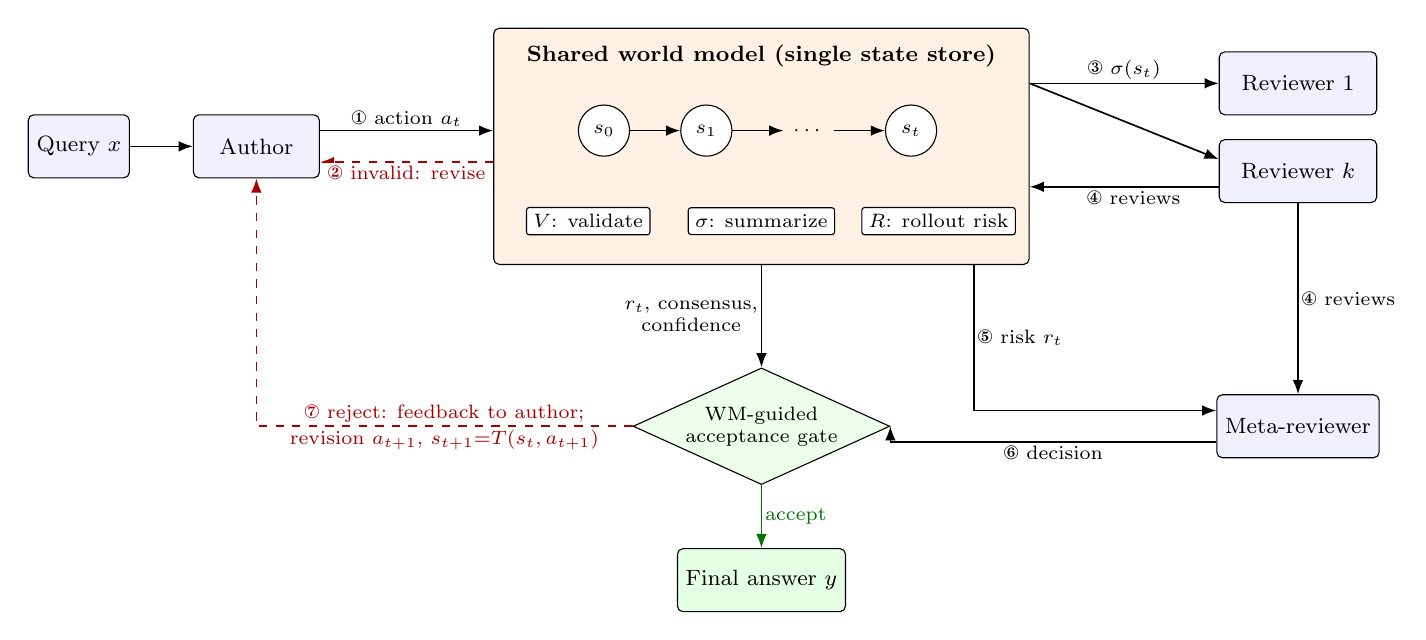
\begin{tikzpicture}[node distance=7mm and 12mm]
\node[agent] (q) {Query $x$};
\node[agent, right=8mm of q, minimum width=16mm] (a) {Author};
\node[wm, right=22mm of a, minimum width=68mm, minimum height=30mm] (w) {};
\node[ttl, anchor=north] at ([yshift=-1mm]w.north) {Shared world model (single state store)};
\node[st] (s0) at ([xshift=-20mm,yshift=2mm]w.center) {$s_0$};
\node[st] (s1) at ([xshift=-7mm,yshift=2mm]w.center) {$s_1$};
\node[font=\scriptsize] (sd) at ([xshift=6mm,yshift=2mm]w.center) {$\cdots$};
\node[st] (s2) at ([xshift=19mm,yshift=2mm]w.center) {$s_t$};
\draw[flow] (s0) -- (s1); \draw[flow] (s1) -- (sd); \draw[flow] (sd) -- (s2);
\node[op] (v) at ([xshift=-22mm,yshift=-9.5mm]w.center) {$V$: validate};
\node[op] (sg) at ([xshift=0mm,yshift=-9.5mm]w.center) {$\sigma$: summarize};
\node[op] (rr) at ([xshift=22.5mm,yshift=-9.5mm]w.center) {$R$: rollout risk};
\node[agent, right=24mm of w, yshift=8mm, minimum width=20mm] (r1) {Reviewer 1};
\node[agent, below=3mm of r1, minimum width=20mm] (r2) {Reviewer $k$};
\node[gate, below=13mm of w] (g) {WM-guided\\acceptance gate};
\node[agent, minimum width=20mm] (m) at (r2 |- g) {Meta-reviewer};
\node[agent, below=8mm of g, fill=green!10] (out) {Final answer $y$};

\draw[flow] (q) -- (a);
\draw[flow] ([yshift=2mm]a.east) -- node[lbl, above] {\ding{172} action $a_t$} ([yshift=2mm]a.east -| w.west);
\draw[fb] ([yshift=-2mm]a.east -| w.west) -- node[lbl, below] {\ding{173} invalid: revise} ([yshift=-2mm]a.east);
\draw[flow] ([yshift=8mm]w.east) -- node[lbl, above] {\ding{174} $\sigma(s_t)$} (r1.west);
\draw[flow] ([yshift=8mm]w.east) -- ([yshift=1.5mm]r2.west);
\draw[flow] ([yshift=-2mm]r2.west) -- node[lbl, below, pos=0.45] {\ding{175} reviews} ([yshift=-2mm]r2.west -| w.east);
\draw[flow] (r2) -- node[lbl, right] {\ding{175} reviews} (m);
\draw[flow] ([xshift=27mm]w.south) |- node[lbl, pos=0.25, right] {\ding{176} risk $r_t$} ([yshift=2mm]m.west);
\draw[flow] ([yshift=-2mm]m.west) -- node[lbl, below, pos=0.5] {\ding{177} decision} ([yshift=-2mm]m.west -| g.east) -- (g.east);
\draw[flow] (w.south) -- node[lbl, left] {$r_t$, consensus,\\confidence} (g.north);
\draw[flow, green!45!black] (g) -- node[lbl, right] {accept} (out);
\draw[fb] (g.west) -| node[lbl, pos=0.25, above] {\ding{178} reject: feedback to author;}  node[lbl, pos=0.25, below] {revision $a_{t+1}$, $s_{t+1}{=}T(s_t,a_{t+1})$} (a.south);
\end{tikzpicture}
}
    \caption{Centralized world-model coordination. All agents read from and write to one shared state store; the world model validates each action, distributes the state summary, computes the trajectory risk from the reviews, and gates acceptance.}
    \label{fig:centralized}
\end{figure*}

\subsubsection{Peer-to-peer coordination}
In the peer architecture (Fig.~\ref{fig:peer}) there is no shared state store. Every agent owns a local world-model instance.
The author commits and validates its candidates in its local instance and sends the resulting summary to the reviewers as part of its message; each reviewer and the meta-reviewer mirror the received information into their own local instances.
The meta-reviewer's local world model has no access to a shared review record and therefore computes only a local risk (Eq.~\eqref{eq:risk} without the review-dependent terms, with base level 0.5), which is reported in the meta-reviewer prompt.
There is no global gate: a candidate is accepted as soon as the meta-reviewer decides ``right''.
Peer coordination is thus the lighter mechanism. It keeps explicit state tracking and validation on the author side but leaves the acceptance decision to the agents, whereas centralized coordination adds a conservative, state-level check that can overrule them.

\begin{figure*}[!t]
    \centering
    \resizebox{0.95\textwidth}{!}{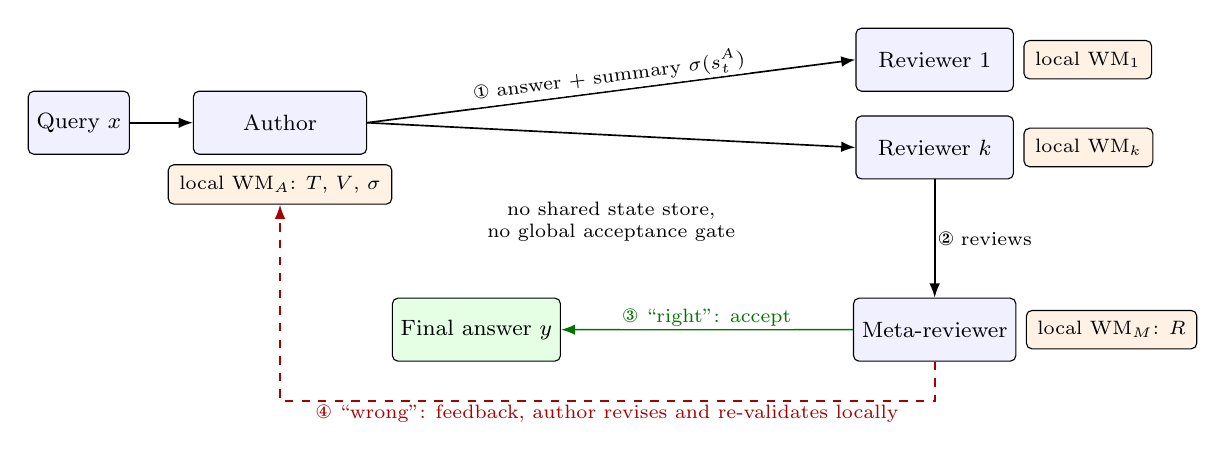
\begin{tikzpicture}[node distance=7mm and 12mm]
\node[agent] (q) {Query $x$};
\node[agent, right=8mm of q, minimum width=22mm] (a) {Author};
\node[wm, below=1.2mm of a, minimum width=22mm, font=\scriptsize] (wa) {local WM$_A$: $T$, $V$, $\sigma$};
\node[agent, right=62mm of a, yshift=8mm, minimum width=20mm] (r1) {Reviewer 1};
\node[wm, right=1.2mm of r1, font=\scriptsize] (w1) {local WM$_1$};
\node[agent, below=3mm of r1, minimum width=20mm] (r2) {Reviewer $k$};
\node[wm, right=1.2mm of r2, font=\scriptsize] (w2) {local WM$_k$};
\node[agent, below=15mm of r2, minimum width=20mm] (m) {Meta-reviewer};
\node[wm, right=1.2mm of m, font=\scriptsize] (wmm) {local WM$_M$: $R$};
\node[agent, fill=green!10] (out) at ($(a |- m)!0.3!(m)$) {Final answer $y$};
\node[font=\scriptsize, align=center, text width=44mm] at ($(a.east)!0.5!(r2.west)+(0,-11mm)$) {no shared state store,\\no global acceptance gate};

\draw[flow] (q) -- (a);
\draw[flow] (a.east) -- node[lbl, above, sloped] {\ding{172} answer + summary $\sigma(s^{A}_t)$} (r1.west);
\draw[flow] (a.east) -- (r2.west);
\draw[flow] (r2) -- node[lbl, right] {\ding{173} reviews} (m);
\draw[flow, green!45!black] (m.west) -- node[lbl, above] {\ding{174} ``right'': accept} (out.east);
\draw[fb] (m.south) -- ++(0,-5mm) -| node[lbl, pos=0.25, below] {\ding{175} ``wrong'': feedback, author revises and re-validates locally} (wa.south);
\end{tikzpicture}
}
    \caption{Peer-to-peer world-model coordination. Each agent keeps a local world-model replica; state summaries travel inside messages, and acceptance follows the meta-reviewer's decision.}
    \label{fig:peer}
\end{figure*}

\subsection{World-Model--Guided Acceptance}
\label{sec:gate}

In centralized mode a candidate that the meta-reviewer judges ``right'' is accepted only if it also passes the following gate.
Let \(\kappa\) be the number of reviewers counted as agreeing with the candidate (a reviewer agrees if its review has positive polarity or its reliability exceeds 0.7).
The risk is first adjusted by lexical cues in the meta-review, \(r'_t = \mathrm{clip}_{[0,1]}(r_t + \Delta_{\mathrm{meta}})\), where \(\Delta_{\mathrm{meta}}\in[-0.15,+0.25]\) is positive when the meta-review mentions flaws or concerns and negative when it states that the answer is clearly correct.
The \emph{effective risk} combines the adjusted risk with reviewer reliability,
\begin{equation}
\tilde r_t = 0.7\, r'_t + 0.3\,(1-\bar c),
\end{equation}
and is compared with a length-aware threshold \(\theta = \theta_0 + \min(0.12,\ L/900)\), where \(L\) is the number of words in the candidate.
The candidate is accepted if either
\begin{align}
&\tilde r_t \le \theta \ \wedge\ \kappa \ge \kappa_{\min} \ \wedge\ \bar c > c_{\min}, \quad\text{or} \label{eq:gateA}\\
&\kappa = k \ \wedge\ \bar c > c_{\mathrm{full}} \ \wedge\ \tilde r_t \le r_{\mathrm{cap}}. \label{eq:gateB}
\end{align}
Otherwise the meta-review is returned to the author as feedback, the author revises, and the revision is committed as a new state.
Table~\ref{tab:hyper} lists the gate hyperparameters. They are defined per answer format rather than per dataset and were fixed before the experiments reported in this paper.

\begin{table}[!t]
\caption{Acceptance-gate hyperparameters (centralized mode)}
\label{tab:hyper}
\centering
\footnotesize
\setlength{\tabcolsep}{3pt}
\begin{tabular}{lccccc}
\toprule
Task family & $\theta_0$ & $\kappa_{\min}$ & $c_{\min}$ & $c_{\mathrm{full}}$ & $r_{\mathrm{cap}}$ \\
\midrule
\makecell[l]{GSM8K, SVAMP,\\GSM-Hard, StrategyQA} & 0.28 & 2 & 0.65 & 0.80 & 0.45 \\
CIAR & 0.35 & 1 & 0.60 & 0.75 & 0.50 \\
MMLU subsets & 0.38 & 1 & 0.58 & 0.72 & 0.52 \\
\bottomrule
\end{tabular}
\end{table}

\subsection{Overall Procedure}

Algorithm~\ref{alg:wm-agent} summarizes one run. The same procedure covers both architectures; they differ in where the state lives and in the acceptance test of line~\ref{line:accept}.

\begin{algorithm}[t]
\caption{World-Model--Guided Multi-Agent Reasoning}
\label{alg:wm-agent}
\begin{algorithmic}[1]
\REQUIRE Query \(x\), reviewers \(k\), maximum review rounds \(N\)
\ENSURE Final answer \(y\)
\STATE \(s \leftarrow T(\varnothing, \langle\textsc{init}, x\rangle)\)
\STATE Author drafts candidate \(c\); \(a \leftarrow \langle\textsc{draft}, c\rangle\); \(s \leftarrow T(s, a)\)
\IF{\(V(s,a)\) fails}
    \STATE Author re-submits \(c\) given the validator hint; \(s \leftarrow T(s, \langle\textsc{revalidated}, c\rangle)\)
\ENDIF
\FOR{\(n = 1,\ldots,N\)}
    \STATE Each reviewer evaluates \(c\) given \(\sigma(s)\) \(\rightarrow\) reviews \(\mathcal{F}\)
    \STATE \(r \leftarrow R(s, \mathcal{F})\) \COMMENT{trajectory risk, Eq.~\eqref{eq:risk}}
    \STATE Meta-reviewer decides \(d\in\{\text{right},\text{wrong}\}\) given \(c, \mathcal{F}, r\)
    \IF{\(d=\text{right}\) \AND \textsc{Accept}\((r,\mathcal{F})\)} \label{line:accept}
        \RETURN answer of \(c\)
    \ENDIF
    \IF{\(n<N\)}
        \STATE Author revises \(c\) given the meta-review; \(a \leftarrow \langle\textsc{revision}, c\rangle\); \(s \leftarrow T(s,a,n)\)
        \STATE Re-submit once if \(V(s,a)\) fails
    \ENDIF
\ENDFOR
\RETURN answer of the last candidate \(c\)
\end{algorithmic}
\vspace{2pt}
{\footnotesize \textsc{Accept} is Eqs.~\eqref{eq:gateA}--\eqref{eq:gateB} in centralized mode and always true in peer mode.}
\end{algorithm}

\subsection{Coordination Uncertainty Index}
\label{sec:cui}

To characterize when each architecture is preferable we define the \emph{Coordination Uncertainty Index} (CUI), a dataset-level statistic computed from the logs of the first review round.
It is inspired by information-theoretic notions of uncertainty~\cite{shannon1948mathematical} and aggregates four signals of how hard it is for the agents to agree on a stable shared state.
For a dataset \(D\) with \(N\) tasks:

\begin{itemize}
\item \textbf{Reviewer belief entropy.} Let \(p^{(i)}\) be the fraction of reviewers whose decision on task \(i\) is ``right''. Then
\(H_{\mathrm{rev}} = \tfrac1N\sum_i \big[-p^{(i)}\log p^{(i)} - (1-p^{(i)})\log(1-p^{(i)})\big]\).
\item \textbf{Confidence dispersion.} \(V_{\mathrm{conf}} = \tfrac1N\sum_i \mathrm{Var}(c^{(i)}_1,\ldots,c^{(i)}_k)\), the variance of the reviewers' reliability scores.
\item \textbf{Risk instability.} \(V_{\mathrm{risk}} = \tfrac1N\sum_i \mathrm{Var}(r^{(i)}_1,\ldots,r^{(i)}_{n_i})\), the variance of the trajectory risk (Eq.~\eqref{eq:risk}) over the \(n_i\) review rounds of task \(i\) (zero for single-round tasks).
\item \textbf{Answer entropy.} \(H_{\mathrm{ans}}\) is the mean Shannon entropy of the multiset of normalized final answers proposed for a task by the author, the reviewers, and the meta-reviewer.
\end{itemize}

Each component is min--max normalized over the pool of datasets under study (denoted by a hat), and the index is their unweighted mean:
\begin{equation}
\label{eq:cui}
U(D) = \tfrac14\big(\hat H_{\mathrm{rev}} + \hat V_{\mathrm{conf}} + \hat V_{\mathrm{risk}} + \hat H_{\mathrm{ans}}\big).
\end{equation}
We use equal weights to avoid fitting additional free parameters on a small number of datasets.
Because of the normalization, \(U(D)\) is a \emph{relative} index: it ranks the datasets of a pool by coordination uncertainty, and a threshold \(\tau\) is meaningful only with respect to that pool.
Unless stated otherwise, the CUI is computed from peer-mode logs, which are the cheapest to obtain.

\section{Experimental Setup}
\label{sec:setup}

\subsection{Backbones and Inference Configuration}
\label{sec:llm}

All agents in a run share one backbone LLM. To test whether the findings depend on the backbone we use four OpenAI models that differ in capability: \texttt{gpt-3.5-turbo} (snapshot \texttt{gpt-3.5-turbo-0125}), \texttt{gpt-4o-mini} (snapshot \texttt{gpt-4o-mini-2024-07-18}), \texttt{gpt-4.1-nano} (snapshot \texttt{gpt-4.1-nano-2025-04-14}), and \texttt{gpt-4.1-mini} (snapshot \texttt{gpt-4.1-mini-2025-04-14}).
All models are accessed through the OpenAI Chat Completions API.
Every call uses temperature \(1.0\), the API defaults for nucleus sampling and output length, a fresh random seed, and \texttt{logprobs} enabled; the token log-probabilities are used only to compute the reviewer reliability score of Section~\ref{sec:wm}.
No system prompt, tool, or retrieval component is used.
All coordination strategies and all baselines use the same backbone, the same decoding configuration, and the same answer format within a comparison, so that differences in accuracy are attributable to the coordination strategy.
The reviewer-style configurations use one author, \(k=2\) reviewers, one meta-reviewer, and at most \(N=3\) review rounds.

\subsection{Benchmarks}

We evaluate on eight reasoning benchmarks (Table~\ref{tab:dataset_overview}):
\textbf{GSM8K}~\cite{cobbe2021gsm8k}, grade-school math word problems;
\textbf{SVAMP}~\cite{patel2021svamp}, arithmetic word problems with structural perturbations;
\textbf{GSM-Hard}~\cite{gao2023pal}, GSM8K problems with numbers replaced by large values;
\textbf{CIAR}~\cite{liang2024mad}, counter-intuitive arithmetic reasoning problems;
\textbf{StrategyQA}~\cite{geva2021strategyqa}, yes/no questions that require implicit multi-hop reasoning;
and three subsets of \textbf{MMLU}~\cite{hendrycks2021mmlu}: \emph{elementary mathematics}, \emph{moral scenarios}, and \emph{professional law}.
The first four benchmarks have numeric answers (scored correct within an absolute tolerance of \(0.01\)); the others are multiple-choice or binary and are scored by exact match of the selected option.

For each benchmark we fix one list of 50 question indices (all 48 questions for CIAR), sampled once, and evaluate \emph{every} method and \emph{every} backbone on exactly these questions, giving 398 questions per backbone.
The three reviewer-style configurations are run with all four backbones in two independent runs (1{,}592 paired questions, 3{,}184 runs per configuration in total), the external baselines once with \texttt{gpt-4.1-mini} and \texttt{gpt-4.1-nano}, and the ablations once with \texttt{gpt-4o-mini}, the backbone on which the centralized gate had the largest effect in the first run.
A disjoint set of 30 further questions per benchmark (210 in total; CIAR has no unused questions) is reserved as a development split for the exploratory variants of Sections~\ref{sec:pilot}--\ref{sec:combined}.

\begin{table}[!t]
\caption{Evaluation Benchmarks}
\label{tab:dataset_overview}
\centering
\footnotesize
\setlength{\tabcolsep}{3pt}
\begin{tabular}{llll}
\toprule
Benchmark & Domain & Answer & \#Q \\
\midrule
GSM8K & Math word problems & Numeric & 50 \\
SVAMP & Math word problems & Numeric & 50 \\
GSM-Hard & Math, large numbers & Numeric & 50 \\
MMLU-Elem. & Elementary mathematics & 4-way MC & 50 \\
CIAR & Counter-intuitive arithmetic & Numeric & 48 \\
StrategyQA & Implicit multi-hop QA & Binary & 50 \\
MMLU-Moral & Moral scenarios & 4-way MC & 50 \\
MMLU-Law & Professional law & 4-way MC & 50 \\
\bottomrule
\end{tabular}
\end{table}

\subsection{Compared Methods}

\paragraph{Reviewer-style configurations.}
\emph{Reviewer pipeline} is the message-based author--reviewer--meta-reviewer pipeline of MARS~\cite{wang2025mars} without any world model; it accepts a candidate when the meta-reviewer decides ``right''.
\emph{Ours (Peer)} and \emph{Ours (Centralized)} add the world model of Section~\ref{sec:method} in the two coordination architectures.
The three configurations share all prompts.

\paragraph{External baselines.}
We re-implement six methods in the same evaluation pipeline, with the same backbone and answer format:
\emph{CoT}, a single chain-of-thought call~\cite{wei2022chain};
\emph{Self-Consistency} with five samples and majority voting~\cite{wang2023selfconsistency};
\emph{Self-Reflection}, one answer followed by one self-critique and revision~\cite{madaan2023selfrefine,shinn2023reflexion};
\emph{Multi-Agent Debate} with three agents and two rounds~\cite{du2024improving};
\emph{MAD} with an affirmative debater, a negative debater, and a judge that may stop the debate, for at most three rounds~\cite{liang2024mad};
and \emph{ReConcile} with three agents, at most three discussion rounds, and confidence-weighted voting~\cite{chen2024reconcile}.
ReConcile was proposed for a mixture of different LLMs; to keep the backbone fixed we use its single-backbone variant and omit its ``convincing samples'' component.
We do not include AgentVerse or GPTSwarm as baselines: the former recruits task-specific expert roles and the latter optimizes a graph on a training split, so neither can be reproduced faithfully in a setting with a fixed role set and no training data.

\paragraph{Ablations.}
Starting from the centralized configuration we remove one world-model component at a time:
(i) \emph{w/o shared state summary}: reviewers do not receive \(\sigma(s_t)\);
(ii) \emph{w/o transition validation}: \(V\) is skipped;
(iii) \emph{w/o trajectory risk}: \(R\) is not computed, so the risk is neither shown to the meta-reviewer nor used in the gate (the consensus and reliability conditions remain);
(iv) \emph{w/o WM-guided acceptance}: the gate of Section~\ref{sec:gate} is removed and acceptance follows the meta-reviewer, while state, validation, and risk reporting remain.

\subsection{Metrics and Statistical Analysis}

We report accuracy, the average number of tokens (prompt plus completion) per question, the average number of LLM calls per question, and the average wall-clock time per question.
Because individual benchmarks contain at most 50 questions, per-benchmark differences below roughly 15 percentage points cannot be resolved, and we base our conclusions on comparisons pooled over benchmarks. We accompany accuracy differences with paired tests: for two methods evaluated on the same questions we compute the per-question difference in correctness, a 95\% bootstrap confidence interval of its mean, and a two-sided paired sign-flip permutation test (20{,}000 permutations).
We do not correct for multiple comparisons and therefore treat per-dataset \(p\)-values as descriptive.
Every number in the tables and figures of this paper is generated by a single analysis script from the per-question run logs.


\section{Results}
\label{sec:results}

\subsection{Does the Collective Correct Its Members?}
\label{sec:agreement}

Because the author's first draft is logged in every run, we can measure what the rest of the pipeline contributes within a run, as the change from draft accuracy to final accuracy, together with the first-round acceptance decision.
Table~\ref{tab:gate} reports these quantities for the three reviewer-style configurations and all four backbones, pooled over the two independent runs (796 runs per row).

\begin{table*}[!t]
\caption{Within-run effect of each configuration (398 questions $\times$ 2 runs per row). Draft/Final: accuracy (\%) of the author's first draft and of the returned answer. W$\to$R / R$\to$W: share of runs (\%) whose answer changes from wrong to right / right to wrong. Pass: share (\%) of correct and of incorrect drafts accepted in the first round. Repaired: share (\%) of incorrect drafts not accepted in the first round that end correct (count of such drafts in parentheses).}
\label{tab:gate}
\small
\setlength{\tabcolsep}{4.5pt}
\resizebox{\linewidth}{!}{\begin{tabular}{ll ccc cc cc c cc}
\toprule
 & & \multicolumn{3}{c}{Accuracy} & \multicolumn{2}{c}{Flips} & \multicolumn{2}{c}{Pass in round 1} & & & \\
\cmidrule(lr){3-5}\cmidrule(lr){6-7}\cmidrule(lr){8-9}
Backbone & Configuration & Draft & Final & Net & W$\to$R & R$\to$W & Correct & Incorrect & Repaired & Rounds & Tokens \\
\midrule
\tabinput{tables/gate.tex}
\bottomrule
\end{tabular}}
\end{table*}

\paragraph{Without an external gate, review is close to a rubber stamp.}
In the message-based reviewer pipeline, 80--97\% of incorrect drafts are accepted in the first round because the meta-reviewer judges them ``right''; the average number of review rounds is between 1.01 and 1.15, and the net change from draft to final accuracy is between \(+0.3\) and \(+1.9\) points (significant for GPT-4.1-nano only, \(p=0.009\)).
The four-agent pipeline therefore returns, in the large majority of cases, the answer that a single call would have produced.
The strongest backbone is the most extreme case: with GPT-4.1-mini 97\% of incorrect drafts pass, the reviewers almost never disagree with the author, and in 796 runs the pipeline changes four answers.

\paragraph{Explicit state alone does not change this.}
The peer-to-peer configuration adds explicit state tracking and validation on the author side and a state summary in every reviewer prompt, but leaves acceptance to the agents.
Its statistics are those of the reviewer pipeline: 81--94\% of incorrect drafts pass, rounds average 1.01--1.12, and the net gain is \(+0.8\) to \(+1.3\) points, not significant in any case.

\paragraph{How large is run-to-run variation?}
Table~\ref{tab:repcons} reports the accuracy of each configuration in each of the two runs separately.
The same configuration on the same 398 questions differs between runs by 1.9 points on average and by up to 4.0 points, because every call samples at temperature 1.0.
This is the yardstick against which the remaining comparisons must be read: a single-run difference of a few points between two configurations carries no information, and we therefore base all conclusions on the pooled two-run comparisons.

\begin{table}[!t]
\caption{Accuracy (\%) of each configuration in the two independent runs (398 questions each), and the centralized$-$reviewer difference in each run.}
\label{tab:repcons}
\footnotesize
\setlength{\tabcolsep}{4pt}
\begin{tabular}{l ccc ccc cc}
\toprule
 & \multicolumn{3}{c}{Run 1} & \multicolumn{3}{c}{Run 2} & \multicolumn{2}{c}{Centr.\ $-$ Rev.} \\
\cmidrule(lr){2-4}\cmidrule(lr){5-7}\cmidrule(lr){8-9}
Backbone & Rev. & Peer & Centr. & Rev. & Peer & Centr. & Run 1 & Run 2 \\
\midrule
\tabinput{tables/rep_consistency.tex}
\bottomrule
\end{tabular}
\end{table}

\begin{figure*}[!t]
\centering
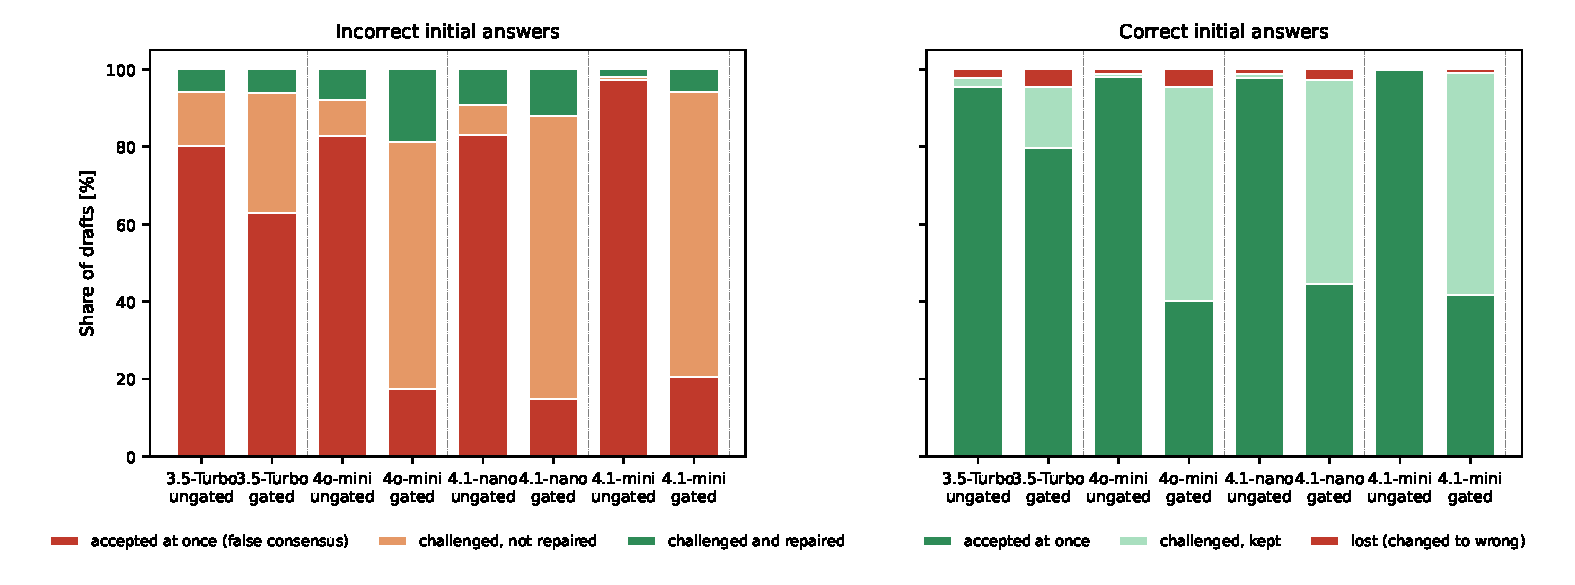
\includegraphics[width=0.95\textwidth]{figures/correction_flow.pdf}
\Description{Stacked bar charts for four backbones under ungated and gated configurations. Left: incorrect initial answers split into accepted at once, challenged but not repaired, and challenged and repaired. Right: correct initial answers split into accepted, challenged but kept, and lost.}
\caption{Where collective correction succeeds and fails. Fate of incorrect (left) and correct (right) initial answers under the ungated reviewer pipeline and the centralized gate, for each backbone (both runs pooled). An incorrect draft is either accepted at once (false consensus), challenged but not repaired, or challenged and repaired; a correct draft is accepted, challenged but kept, or lost.}
\label{fig:flow}
\end{figure*}

Fig.~\ref{fig:flow} shows the same data as a flow.
Under the ungated pipeline the left panel is almost entirely ``false consensus'': the reviewers and the meta-reviewer confirm the incorrect draft, and the few drafts that are challenged are repaired about half of the time.
These numbers are the central empirical fact of the paper: a reviewer-style LLM collective whose members share a backbone and read the author's draft behaves, to a first approximation, as a single agent.
We read the rest of the results through a three-stage decomposition of what such a collective would have to do to correct a member: \emph{detect} that a draft may be wrong, \emph{challenge} it (withhold acceptance and send it back), and \emph{repair} it (produce a correct alternative).
In the ungated pipeline the collective fails at the first stage.

\subsection{Interventions: Detect, Challenge, Repair}
\label{sec:mechanisms}

\subsubsection{Centralized world-model gating}
\label{sec:main_results}

In the centralized configuration a candidate is accepted only if the world model's state-level test (Section~\ref{sec:gate}) is satisfied, whatever the meta-reviewer says.
This moves the \emph{detect} and \emph{challenge} stages out of the agents' hands; the \emph{repair} stage remains with the author.
Table~\ref{tab:main_results} reports per-benchmark accuracy for all configurations and Table~\ref{tab:pooled} the pooled paired comparisons.

\begin{table*}[!t]
\caption{Accuracy (\%) of the three reviewer-style configurations on identical questions (50 per benchmark, 48 for CIAR), averaged over two independent runs. Rev.: message-based reviewer pipeline. Bold: best per backbone and benchmark. The last row is the macro-average over benchmarks.}
\label{tab:main_results}
\small
\setlength{\tabcolsep}{3.5pt}
\resizebox{\linewidth}{!}{\begin{tabular}{l ccc ccc ccc ccc}
\toprule
 & \multicolumn{3}{c}{GPT-3.5-Turbo} & \multicolumn{3}{c}{GPT-4o-mini} & \multicolumn{3}{c}{GPT-4.1-nano} & \multicolumn{3}{c}{GPT-4.1-mini} \\
\cmidrule(lr){2-4}\cmidrule(lr){5-7}\cmidrule(lr){8-10}\cmidrule(lr){11-13}
Benchmark & Rev. & Peer & Centr. & Rev. & Peer & Centr. & Rev. & Peer & Centr. & Rev. & Peer & Centr. \\
\midrule
\tabinput{tables/main_results.tex}
\bottomrule
\end{tabular}}
\end{table*}

\begin{table*}[!t]
\caption{Pooled paired comparisons over all questions (per-question accuracy averaged over the two runs). Differences are in accuracy points with 95\% bootstrap confidence intervals; $p$: two-sided paired permutation test.}
\label{tab:pooled}
\small
\setlength{\tabcolsep}{4pt}
\resizebox{\linewidth}{!}{\begin{tabular}{l c ccc cc cc cc}
\toprule
 & & \multicolumn{3}{c}{Accuracy (\%)} & \multicolumn{2}{c}{Peer $-$ Rev.} & \multicolumn{2}{c}{Centr. $-$ Rev.} & \multicolumn{2}{c}{Centr. $-$ Peer} \\
\cmidrule(lr){3-5}\cmidrule(lr){6-7}\cmidrule(lr){8-9}\cmidrule(lr){10-11}
Backbone & $n$ & Rev. & Peer & Centr. & $\Delta$ [95\% CI] & $p$ & $\Delta$ [95\% CI] & $p$ & $\Delta$ [95\% CI] & $p$ \\
\midrule
\tabinput{tables/pooled.tex}
\bottomrule
\end{tabular}}
\end{table*}

\paragraph{The gate intervenes, but with little discrimination.}
With the three more recent backbones the gate reduces the first-round acceptance of incorrect drafts to 15--21\% (Table~\ref{tab:gate}).
It does so mainly by being strict rather than selective: it also withholds acceptance from 55--60\% of \emph{correct} drafts, and thus roughly doubles the number of review rounds for correct and incorrect drafts alike.
With GPT-3.5-Turbo the same gate, with the same thresholds, is lenient instead (80\% of correct and 63\% of incorrect drafts pass): a gate built on reviewer confidence and review wording does not transfer across backbones without recalibration.

\paragraph{Detection is not correction.}
The gate thus has some detection capability (it intercepts 79--85\% of incorrect drafts on the three more recent backbones, right panel of Fig.~\ref{fig:flow}) but poor specificity (it also intercepts 55--60\% of correct ones), and the repair stage is where the intervention fails.
Of the incorrect drafts that the gate sends back, only 7\% (GPT-4.1-mini) to 23\% (GPT-4o-mini) end with a correct answer, and some initially correct answers are lost on the way (0.8--3.3\% of runs).
The net within-run gain of the centralized configuration is \(0.0\), \(+1.8\), \(+1.4\), and \(+0.4\) points for the four backbones, not significant in any case, and no larger than the gain of the ungated reviewer pipeline on the same backbone (\(+1.4\), \(+1.3\), \(+1.9\), \(+0.3\)).
The pooled paired differences to the reviewer pipeline (Table~\ref{tab:pooled}) are \(-0.5\), \(+0.8\), \(+1.8\), and \(-0.5\) points, all with confidence intervals that include zero, and \(+0.4\) points overall (\(p=0.58\)).

\paragraph{A cautionary tale about single runs.}
In the first run alone, the centralized configuration with GPT-4o-mini gained \(+4.3\) points over its drafts (\(p=0.012\)) and \(+4.0\) points over the reviewer pipeline (\(p=0.033\)), was at least as accurate as the pipeline on all eight benchmarks, and would have been reported as a clear positive result.
In the second run it \emph{lost} \(0.8\) points against its drafts and \(2.5\) points against the pipeline (Table~\ref{tab:repcons}).
Neither run is anomalous; both lie within the run-to-run variation of Table~\ref{tab:repcons}.
We report this explicitly because the earlier version of this study, based on single runs, drew conclusions of exactly this kind.

\paragraph{Cost.}
Table~\ref{tab:efficiency} shows that the peer configuration costs about as much as the reviewer pipeline, whereas the centralized configuration uses \(1.7\times\) (GPT-3.5-Turbo) to \(4.3\times\) (GPT-4.1-mini) the tokens and roughly twice the LLM calls, because the gate triggers additional review rounds; the overhead grows with task difficulty.

\begin{table}[!t]
\caption{Cost per question with GPT-4o-mini: tokens, LLM calls, and wall-clock time (s, measured under concurrent execution). R: reviewer pipeline, P: peer, C: centralized.}
\label{tab:efficiency}
\footnotesize
\setlength{\tabcolsep}{3pt}
\resizebox{\linewidth}{!}{\begin{tabular}{l rrr rrr rrr}
\toprule
 & \multicolumn{3}{c}{Tokens} & \multicolumn{3}{c}{Calls} & \multicolumn{3}{c}{Time} \\
\cmidrule(lr){2-4}\cmidrule(lr){5-7}\cmidrule(lr){8-10}
Benchmark & R & P & C & R & P & C & R & P & C \\
\midrule
\tabinput{tables/efficiency.tex}
\bottomrule
\end{tabular}}
\end{table}

\subsection{Ablation of World-Model Components}
\label{sec:ablation}

To see which component of the centralized configuration is responsible for its behaviour we remove them one at a time with GPT-4o-mini (Table~\ref{tab:ablation}).
Each variant is run once on the same 398 questions; for comparability the table shows the \emph{first} run of the two reference configurations, which were run in the same batch.

\begin{table*}[!t]
\caption{Ablation with GPT-4o-mini (398 questions per row, single run). Columns as in Table~\ref{tab:gate}; $\Delta$ Full: paired difference in final accuracy to the full centralized configuration in the same run (points, $p$ of the paired permutation test in parentheses).}
\label{tab:ablation}
\footnotesize
\setlength{\tabcolsep}{3pt}
\resizebox{\linewidth}{!}{\begin{tabular}{l ccc cc cc c cc c}
\toprule
 & \multicolumn{3}{c}{Accuracy} & \multicolumn{2}{c}{Flips} & \multicolumn{2}{c}{Pass in round 1} & & & & \\
\cmidrule(lr){2-4}\cmidrule(lr){5-6}\cmidrule(lr){7-8}
Configuration & Draft & Final & Net & W$\to$R & R$\to$W & Correct & Incorrect & Repaired & Rounds & Tokens & $\Delta$ Full \\
\midrule
\tabinput{tables/ablation.tex}
\bottomrule
\end{tabular}}
\end{table*}

\paragraph{Accuracy differences are within run-to-run variation.}
The run of the full configuration that serves as reference is the one that gained \(+4.3\) points over its drafts; its second run gained \(-0.8\) (Section~\ref{sec:main_results}).
The four variants gain \(+1.3\) to \(+2.3\) points, i.e., about as much as the ungated pipeline and as the full configuration in its second run.
We therefore do not read the \(\Delta\)~Full column as component contributions: the one nominally significant entry (without the state summary, \(-3.8\) points, \(p=0.02\)) is of the size of the difference between the two runs of the unmodified system.
Running each variant repeatedly would be required to resolve accuracy effects of this size, and the main-result experiment suggests there are none to resolve.

\paragraph{Behaviour and cost are stable and informative.}
The behavioural columns do not depend on the sampling of drafts in the same way, and they tell a consistent story.
Removing the state summary, validation, or the risk estimate leaves the gate's behaviour unchanged: 39--43\% of correct and 14--19\% of incorrect drafts pass, rounds stay at 2.3, and tokens at 15--16k.
Transition validation in particular changes nothing, which is expected since its lexicon-based checks fire rarely.
The variant \emph{without the acceptance gate}, in which the world model still validates, summarizes, and reports the risk to the meta-reviewer but acceptance follows the meta-reviewer's verdict, is the informative one: reporting the risk lowers the first-round acceptance of incorrect drafts from 85\% to 78\% while 97\% of correct drafts still pass, at 1.08 rounds and \(4.8\)k tokens---a third of the cost of gating.
Whatever behavioural effect the full gate has on the collective's willingness to reconsider is thus obtained largely by making the risk visible, and the forced additional rounds (which cost roughly 11k tokens per question) do not turn that reconsideration into measurable accuracy.

\subsection{Exploratory Variant: An Answer-Agreement Gate}
\label{sec:pilot}

The diagnosis of Section~\ref{sec:gate_results} suggests two changes: base the acceptance decision on evidence that is more directly tied to correctness than the reviewers' stated opinions, and give the author more to work with when a draft is sent back.
We tested one simple instantiation on a development split that is disjoint from all questions used above (30 further questions from each benchmark except CIAR, which has no unused questions; 210 questions; GPT-4.1-mini, the backbone on which the centralized gate was least effective).
In this variant there is no meta-reviewer and no risk function. Each reviewer still solves the problem itself, and a draft is accepted if and only if the final answers of all reviewers equal the author's answer. On disagreement the author receives the reviewers' complete solutions and is asked to locate the step at which they diverge before answering again; if no agreement is reached after three rounds, the majority answer is returned.
This experiment is exploratory: it was designed after the main results were known and was run once.

\begin{table}[!t]
\caption{Exploratory Comparison on the Development Split (210 Questions, GPT-4.1-mini). Columns as in Table~\ref{tab:gate}.}
\label{tab:pilot}
\centering
\scriptsize
\setlength{\tabcolsep}{2.5pt}
\resizebox{\linewidth}{!}{\begin{tabular}{l ccc cc c r}
\toprule
 & \multicolumn{3}{c}{Accuracy} & \multicolumn{2}{c}{Pass in round 1} & & \\
\cmidrule(lr){2-4}\cmidrule(lr){5-6}
Configuration & Draft & Final & Net & Correct & Incorr. & Repaired & Tokens \\
\midrule
Reviewer pipe. & 80.5 & 81.4 & $+1.0$ & 100 & 95 & 100 (2) & 3.4k \\
Centralized & 83.8 & 86.2 & $+2.4$ & 44 & 21 & 19 (27) & 14.6k \\
Agreement gate & 83.3 & 85.2 & $+1.9$ & 98 & 80 & 71 (7) & 2.3k \\
\bottomrule
\end{tabular}}
\end{table}

Table~\ref{tab:pilot} shows that the agreement gate fixes one of the two weaknesses and exposes the other.
It is far more selective than the risk-based gate: it accepts 98\% of correct drafts in the first round (against 44\%), so it adds almost no rounds, and it uses 0.66 times the tokens of the reviewer pipeline and 0.15 times those of the centralized configuration.
When it does block an incorrect draft, the author repairs it in five of seven cases, compared with five of 27 for the centralized configuration, which indicates that showing the author concrete alternative solutions is more effective than returning a meta-review.
Its within-run gain (\(+1.9\) points) is comparable to that of the centralized configuration (\(+2.4\)); neither is significant on 210 questions (\(p=0.22\) and \(p=0.06\)).
All three configurations were run once on this split, so, as Table~\ref{tab:repcons} shows for the main split, accuracy differences of this size are within run-to-run variation; the behavioural columns (acceptance and repair rates, rounds, tokens) are the robust content of the table.

The remaining weakness is recall: 80\% of incorrect drafts still pass, because in 28 of 35 cases both reviewers arrive at the same incorrect answer as the author.
The errors of agents that share a backbone are strongly correlated, and in our pipeline the reviewer prompt also contains the author's draft, which may anchor the reviewers despite the instruction to solve the problem first.
An acceptance test based on agreement can therefore only be as good as the independence of the solvers.
Reviewers that never see the draft, and solvers drawn from different backbones as in ReConcile~\cite{chen2024reconcile}, are the obvious next steps; we leave them to future work and do not draw conclusions about accuracy from this exploratory comparison.

\subsection{Testing the Independence Explanation}
\label{sec:independence}

If correlated errors are the obstacle, then making the reviewers more independent should reduce false consensus even without changing the gate.
Two things could make the reviewers of Section~\ref{sec:pilot} non-independent: they share the author's backbone, and their prompt contains the author's draft (with the instruction to solve the problem first).
We varied both, on the same development split and with the same agreement gate: \emph{blind} reviewers never see the draft and simply solve the problem; \emph{heterogeneous} reviewers use a different backbone (GPT-4o-mini) while the author keeps GPT-4.1-mini; and a variant combines both.
Each variant was run once, and the blind same-backbone variant a second time (Table~\ref{tab:independence}).

\begin{table}[!t]
\caption{Independence interventions on the development split (210 questions, author GPT-4.1-mini; one run each, two for the blind variant). Reproduce: share of incorrect drafts for which \emph{both} reviewers independently give the author's wrong answer. Rev.\ acc.: accuracy of the reviewers' own first-round answers. Other columns as in Table~\ref{tab:gate}.}
\label{tab:independence}
\footnotesize
\setlength{\tabcolsep}{2.5pt}
\resizebox{\linewidth}{!}{\begin{tabular}{l cc c cc cc c c r}
\toprule
 & \multicolumn{2}{c}{Reviewers} & & \multicolumn{2}{c}{Pass in round 1} & & & & & \\
\cmidrule(lr){2-3}\cmidrule(lr){5-6}
Variant & see draft & backbone & Rev.\ acc. & Correct & Incorr. & Reproduce & Repaired & Net & Lost & Tokens \\
\midrule
Agreement gate (Sec.~\ref{sec:pilot}) & yes & same & 84 & 98 & 80 & 80 (28/35) & 71 (5/7) & $+1.9$ & 0.5 & 2.3k \\
\quad blind reviewers, run 1 & no & same & 83 & 95 & 48 & 48 (19/40) & 43 (9/21) & $+2.4$ & 1.9 & 2.0k \\
\quad blind reviewers, run 2 & no & same & -- & 95 & 61 & 61 (23/38) & 40 (6/15) & $+1.4$ & 1.4 & 1.7k \\
\quad heterogeneous reviewers & yes & different & 81 & 97 & 84 & 84 (31/37) & 17 (1/6) & $-0.5$ & 1.0 & 2.4k \\
\quad blind + heterogeneous & no & different & 78 & 84 & 42 & 42 (14/33) & 32 (6/19) & $+0.5$ & 2.4 & 2.3k \\
\bottomrule
\end{tabular}}
\end{table}

\paragraph{Exposure to the draft, not the shared backbone, is the dominant measured source of correlation.}
Hiding the draft from same-backbone reviewers reduces the share of incorrect drafts that both reviewers reproduce from 80\% to 48\% in one run and 61\% in a second, and reduces the share that pass the gate by the same amounts, while the reviewers' own accuracy is unchanged (83\% versus 84\%).
Replacing the backbone of the reviewers while still showing them the draft does nothing: a different and somewhat weaker model that reads the author's answer reproduces it in 84\% of the author's failures, if anything more often than the author's own backbone does.
Combining both interventions gives the lowest reproduction rate (42\%) but no clear additional benefit over blind same-backbone reviewers (48--61\%), and the weaker reviewers challenge more correct drafts (16\% versus 5\%).
Reviewer skill is not the explanation: the four reviewer configurations solve the problems with similar accuracy (78--84\%) when their answers are taken on their own.
Our results therefore indicate that, in this setting, exposure to the candidate answer rather than model identity is the dominant source of correlated reviewer errors; we do not claim that this holds for every multi-agent system, but it does show that model heterogeneity alone does not amount to independent judgment.

\paragraph{Where the bottleneck sits: entry into reconsideration, not repair.}
Reading Tables~\ref{tab:pilot} and \ref{tab:independence} together as the three stages of Section~\ref{sec:agreement} locates the failure precisely.
Once an incorrect draft \emph{does} enter reconsideration under the agreement gate, repair is comparatively effective: 5 of 7 such drafts are fixed with draft-exposed reviewers and 9 of 21 with blind reviewers, against 5 of 27 under the risk-based gate, whose challenges carry no alternative solution.
The dominant loss is upstream: with draft-exposed reviewers 80\% of incorrect drafts never enter reconsideration at all, because the reviewers confirm them.
Blind review moves the collective from the first bottleneck to the second: it roughly doubles the share of errors that are challenged (from 20\% to 39--52\% across the two runs), at a cost \emph{below} that of the ungated pipeline (1.7--2.0k versus 3.4k tokens), and the remaining limit is the repair stage, where 40--43\% of challenged errors are fixed in both runs.
The within-run gains (\(+2.4\) and \(+1.4\) points) are within the run-to-run variation documented in Table~\ref{tab:repcons}, and we draw no accuracy conclusion from 210 questions; what the experiment establishes, in both runs, is the mechanism.

\paragraph{What remains.}
The residual 42--61\% overlap of errors under blind review reflects failures that arise even without exposure to the author's draft: for these questions, independent solvers of the same or a similar model make the same mistake.
Such errors are unlikely to be resolved by blinding alone, and they motivate stronger sources of solver diversity---different model families, tools or retrieval, or different reasoning representations---together with an external check that does not rely on agreement at all.

\subsection{Combining Independence With External Oversight}
\label{sec:combined}

The independence interventions of Section~\ref{sec:independence} and the world-model gate of Section~\ref{sec:main_results} address different stages: the former makes the reviewers' evidence more informative, the latter decides what to do with it.
To see whether they complement each other we crossed them on the development split (Table~\ref{tab:combined}).
Blind reviewers in the reviewer pipeline solve the problem without seeing the draft; their review is then formed from whether their answer matches the author's, so that the meta-reviewer, the risk function, and the gate receive input in the usual format.
We vary three further things: whether the meta-reviewer itself sees the draft (a \emph{blind judge} receives only the reviewers' solutions and their match/mismatch reports), whether a rejected author receives the reviewers' solutions in addition to the meta-review (\emph{evidence-preserving repair}), and whether the world-model gate is applied.
The two agreement-gate variants, which replace the meta-reviewer by a rule and return the reviewers' solutions to the author, are repeated for comparison.

\begin{table}[!t]
\caption{Independence and oversight crossed on the development split (210 questions, GPT-4.1-mini, single run). Retained: among incorrect drafts flagged ``wrong'' by at least one reviewer, the number for which the meta-reviewer also decided ``wrong''. Evid.: reviewers' solutions are passed to the author on rejection. Other columns as in Table~\ref{tab:gate}.}
\label{tab:combined}
\footnotesize
\setlength{\tabcolsep}{2.5pt}
\resizebox{\linewidth}{!}{\begin{tabular}{l ccc c c cc c c c r}
\toprule
 & \multicolumn{3}{c}{Sees draft} & & & \multicolumn{2}{c}{Pass in round 1} & & & & \\
\cmidrule(lr){2-4}\cmidrule(lr){7-8}
Configuration & reviewers & judge & evid. & Gate & Retained & Correct & Incorr. & Repaired & Net & Rounds & Tokens \\
\midrule
Reviewer pipeline & yes & yes & no & -- & 2/4 & 100 & 95 & 100 (2/2) & $+1.0$ & 1.01 & 3.4k \\
Centralized WM gate & yes & yes & no & WM & 4/4 & 44 & 21 & 19 (5/27) & $+2.4$ & 2.19 & 14.6k \\
\midrule
Blind reviewers & no & yes & no & -- & 6/19 & 99 & 83 & 50 (3/6) & $+0.5$ & 1.05 & 2.5k \\
Blind reviewers + WM gate & no & yes & no & WM & 6/19 & 68 & 24 & 12 (3/26) & $+0.0$ & 1.70 & 5.4k \\
\midrule
Blind reviewers, blind judge & no & no & no & -- & 12/20 & 98 & 68 & 33 (4/12) & $+1.4$ & 1.12 & 2.8k \\
\quad + evidence-preserving repair & no & no & yes & -- & 7/14 & 97 & 78 & 57 (4/7) & $-1.0$ & 1.08 & 2.6k \\
\quad + evidence-preserving repair + WM gate & no & no & yes & WM & 6/14 & 70 & 19 & 28 (8/29) & $+2.4$ & 1.72 & 6.5k \\
\midrule
Agreement gate (rule, solutions returned) & yes & -- & yes & rule & -- & 98 & 80 & 71 (5/7) & $+1.9$ & 1.06 & 2.3k \\
Agreement gate, blind & no & -- & yes & rule & -- & 95 & 48 & 43 (9/21) & $+2.4$ & 1.24 & 2.0k \\
\bottomrule
\end{tabular}}
\end{table}

\paragraph{Independent evidence is lost again at the aggregation stage.}
Blind reviewers flag 53\% of incorrect drafts (against 10\% when they see the draft), but the meta-reviewer, who does see the draft, overrules them.
The paired transition counts make this precise: of the 36 incorrect drafts in the blind-reviewer pipeline, 19 are flagged by at least one reviewer, and the meta-reviewer retains the flag for 6 of them and overrules it for 13 (retention 32\%); none of the 17 unflagged incorrect drafts is caught by the meta-reviewer on its own.
The judge's overruling is not a calibrated correction of the reviewers: of the 9 \emph{correct} drafts that a blind reviewer flagged, it also overruled 7.
It acts, in effect, as a prior in favour of the draft it has read, discarding about two thirds of reviewer disagreement regardless of whether the disagreement was right.
The same pattern holds in the gated variant (6 of 19 flags retained).
The independence created at the reviewer stage is thus largely undone by a draft-exposed judge at the next stage.

\paragraph{Blinding the judge restores most of the lost independence.}
When the meta-reviewer is also blind, it retains 12 of 20 reviewer flags on incorrect drafts (60\%) instead of 6 of 19 (32\%), and the first-round acceptance of incorrect drafts falls from 83\% to 68\%, with 98\% of correct drafts still accepted.
This turns Principle~2 of Section~\ref{sec:discussion} from an explanation into an intervention result: the loss at the aggregation stage is caused by the judge's exposure to the draft, and is removed by withholding it.
The blind judge does not reach the reviewers' own detection rate (it still overrules 40\% of their flags), so some tendency to accept remains even without exposure.

\paragraph{Carrying the evidence into repair raises the repair rate.}
With a blind judge, passing the reviewers' solutions to a rejected author raises the share of challenged errors that are repaired from 33\% (4 of 12) to 57\% (4 of 7); in the gated chain it raises it from 12\% (3 of 26) to 28\% (8 of 29).
The price is that an author confronted with alternative solutions sometimes abandons a correct answer (2.9\% of runs lost, against 0.5\% without evidence), which is the repair-stage analogue of the specificity problem at the detection stage.

\paragraph{The world-model gate adds specificity, but its repair channel fails without evidence.}
With blind reviewers the gate intercepts 76\% of incorrect drafts while passing 68\% of correct ones, against 44\% with draft-exposed reviewers: the independent evidence makes the gate's risk estimate more selective, and the combination is the most selective detector in the table at a third of the cost of the draft-exposed gate (5.4k versus 14.6k tokens).
But only 3 of the 26 intercepted errors are repaired, because what the author receives after an interception is the meta-review, which was written by a judge who agreed with the draft, rather than the reviewers' alternative solutions.
The rule-based agreement gate with blind reviewers, which returns those solutions, repairs 9 of 21.

\paragraph{What the combination teaches.}
In this setting, oversight and independence do complement each other, but not in the form we first built: the useful oversight is (i) an aggregation step that does not re-expose a judge to the candidate answer and (ii) a repair step that carries the independent solutions to the author.
The full chain---blind reviewers, blind judge, world-model gate, evidence-preserving repair---is the most selective detector in Table~\ref{tab:combined} (19\% of incorrect and 70\% of correct drafts pass) and has the highest repair count of any gated configuration, at less than half the cost of the original gate; the rule-based blind agreement gate remains the cheapest configuration and the one with the highest repair rate, with weaker detection.
The world model's risk estimate contributes selectivity once the evidence feeding it is independent; an LLM meta-reviewer that reads the draft, by contrast, reintroduces exactly the dependence that blinding removed.
Each of these configurations was run once, so we treat the table as a behavioural decomposition and not as an accuracy ranking.

\paragraph{Replication of the two headline variants.}
We ran the blind agreement gate and the blind-reviewer world-model gate a second time on the same 210 questions.
For the world-model gate the behavioural statistics are essentially identical across runs: 68\% and 68\% of correct drafts pass, 24\% and 24\% of incorrect drafts pass, 3 of 26 and 5 of 28 intercepted errors are repaired, and tokens are 5.4k and 5.5k.
For the blind agreement gate the reproduction rate is 48\% in the first run and 61\% in the second (both well below the 80\% of draft-exposed reviewers), the repair rate 43\% and 40\%, and tokens 2.0k and 1.7k.
The direction of every effect reported in this section is the same in both runs; the magnitudes vary by up to 13 points between runs, which is the precision one should attach to single-run cells of Tables~\ref{tab:independence} and \ref{tab:combined}.


\subsection{Falsified Hypotheses: Topology and Uncertainty}
\label{sec:topology}

An earlier version of this study, based on single runs and on comparisons that were not paired, hypothesized that decentralized peer coordination would benefit uncertain tasks, that centralized coordination would benefit structured ones, and that the CUI could predict the preferred regime.
We report the test of these hypotheses in full because their failure is informative: across 32 backbone--benchmark combinations and two runs we find no reliable evidence for either.

\paragraph{Peer versus centralized.}
None of the 32 backbone--benchmark combinations shows a significant difference between the peer and the centralized configuration (smallest \(p=0.19\), uncorrected), and for almost every benchmark the sign of the gap changes from one backbone to the next (on GSM8K it is \(+3\), \(+1\), \(-4\), and \(+2\) points for the four backbones).
In particular, the data do not support a regime in which centralized coordination wins on structured arithmetic benchmarks and peer coordination on ambiguous ones.

\paragraph{The CUI does not select the mode.}
\label{sec:cui_results}
We test the hypothesis of Eq.~\eqref{eq:policy} that datasets with low CUI favor centralized and datasets with high CUI favor peer coordination.
Table~\ref{tab:cui} lists the CUI of every benchmark (computed from that backbone's peer-mode logs) and the gap \(\Delta = \mathrm{Acc}_{\mathrm{peer}} - \mathrm{Acc}_{\mathrm{centralized}}\); Fig.~\ref{fig:cui_regime} plots them.
No correlation is significant: Spearman \(\rho=+0.66\) (\(p=0.08\)) with GPT-3.5-Turbo, \(-0.12\) with GPT-4o-mini, \(+0.28\) with GPT-4.1-nano, and \(+0.20\) with GPT-4.1-mini.
In the first run alone the picture had looked different (\(\rho=+0.74\), \(p=0.036\), with GPT-4.1-mini and \(\rho=-0.58\) with GPT-4o-mini); with the gaps averaged over two runs both associations shrink towards zero.
With eight benchmarks per backbone and gaps that are individually not significant, these correlations give no support for a regime rule.

\begin{table}[!t]
\caption{CUI and peer$-$centralized accuracy gap $\Delta$ (points) per benchmark, and their correlation across the eight benchmarks.}
\label{tab:cui}
\footnotesize
\setlength{\tabcolsep}{2.5pt}
\resizebox{\linewidth}{!}{\begin{tabular}{l cc cc cc cc}
\toprule
 & \multicolumn{2}{c}{3.5-Turbo} & \multicolumn{2}{c}{4o-mini} & \multicolumn{2}{c}{4.1-nano} & \multicolumn{2}{c}{4.1-mini} \\
\cmidrule(lr){2-3}\cmidrule(lr){4-5}\cmidrule(lr){6-7}\cmidrule(lr){8-9}
Benchmark & CUI & $\Delta$ & CUI & $\Delta$ & CUI & $\Delta$ & CUI & $\Delta$ \\
\midrule
\tabinput{tables/cui_compact.tex}
\bottomrule
\end{tabular}}
\end{table}

\begin{figure*}[!t]
\centering
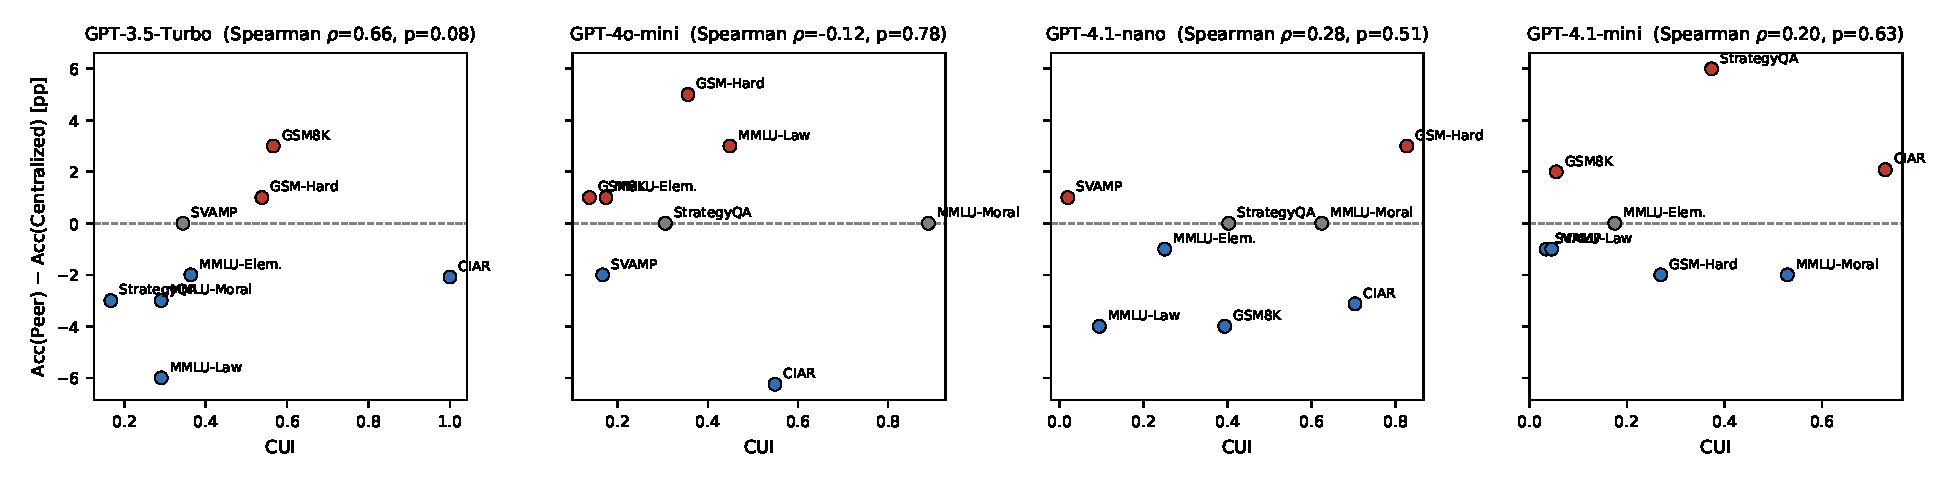
\includegraphics[width=0.95\textwidth]{figures/cui_scatter.pdf}
\Description{Four scatter plots, one per backbone, of the peer minus centralized accuracy gap against the coordination uncertainty index for eight benchmarks.}
\caption{CUI versus the peer$-$centralized accuracy gap. Each point is a benchmark. The sign and strength of the association differ across backbones.}
\label{fig:cui_regime}
\end{figure*}

\begin{figure*}[!t]
\centering
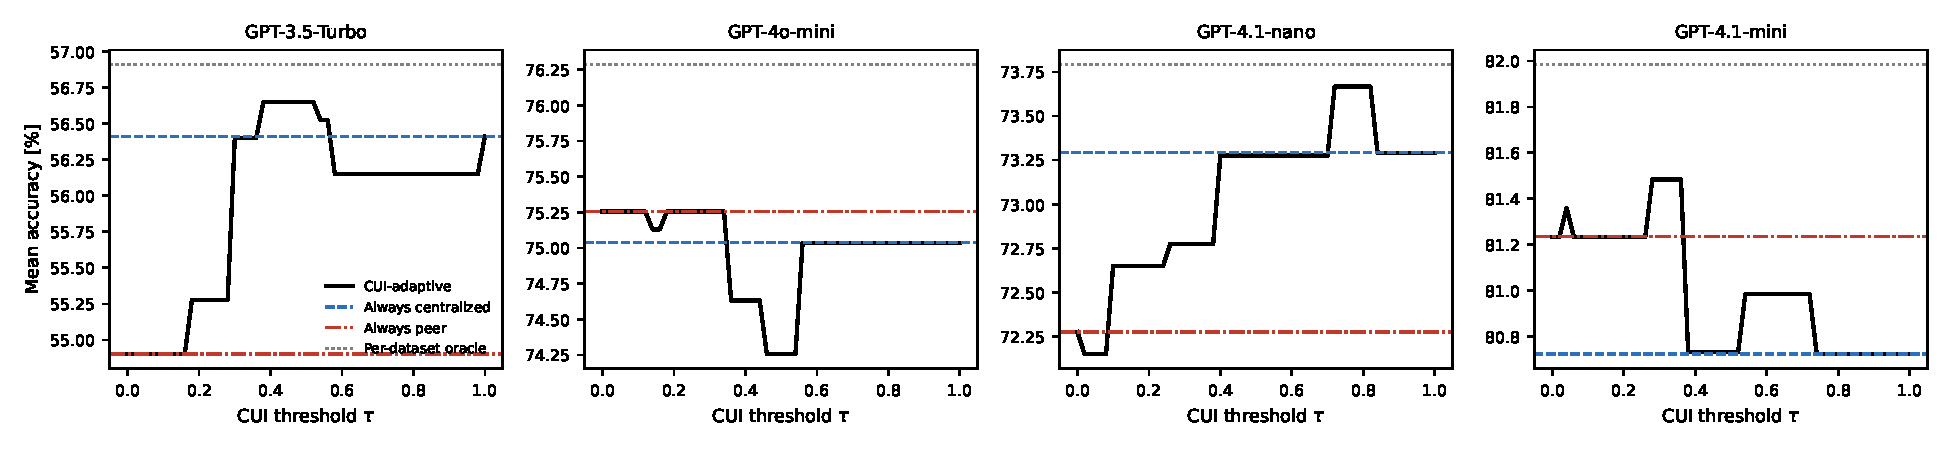
\includegraphics[width=0.95\textwidth]{figures/threshold_sensitivity.pdf}
\Description{Four line plots, one per backbone, of the accuracy of the threshold policy as the threshold varies from zero to one, with horizontal reference lines for the fixed policies and the oracle.}
\caption{Sensitivity of the CUI-adaptive policy to the threshold $\tau$ (macro-averaged accuracy over the eight benchmarks).}
\label{fig:threshold}
\end{figure*}

\paragraph{Threshold sensitivity and held-out evaluation.}
Fig.~\ref{fig:threshold} varies the threshold \(\tau\) of Eq.~\eqref{eq:policy} over its whole range.
The best in-sample threshold improves on the better fixed mode by at most 0.4 points on any backbone, and its location differs across backbones (\([0.38,0.52]\), ``always peer'', \([0.72,0.82]\), \([0.28,0.36]\)).
The per-benchmark oracle is only 0.5--1.0 points above the better fixed mode, so there is little to gain from mode selection even with perfect information.
Out of sample---CUI computed on half of each benchmark's questions, \(\tau\) chosen on the other seven benchmarks, the selected mode scored on the held-out half---the adaptive policy reaches 56.4\%, 75.1\%, 72.8\%, and 82.7\% on the four backbones against 57.2\%, 75.8\%, 74.1\%, and 83.2\% for the better fixed mode: it is worse on all four.
At the level of single tasks and of batches of 5--20 tasks (Table~\ref{tab:fine}), a logistic model predicting ``peer better than centralized'' from the CUI has a benchmark-grouped cross-validated AUC between 0.12 and 0.85 with no consistent trend.
The CUI is a descriptive statistic of reviewer disagreement, not a usable selector.

\paragraph{Why topology does not help.}
The negative result is consistent with the main finding.
Switching from a central state store to local replicas changes who holds the state and who decides, but not what the members are: the same model, in the same context, exposed to the same candidate answer.
A change of communication topology does not create independence, and without independence the collective has nothing new to aggregate.

\begin{table}[!t]
\caption{Predicting ``peer better than centralized'' from the CUI at task and batch level. $R^2$: linear fit of the accuracy gap. AUC: in-sample. CV: cross-validation grouped by benchmark.}
\label{tab:fine}
\footnotesize
\setlength{\tabcolsep}{3pt}
\resizebox{\linewidth}{!}{\begin{tabular}{llccccc}
\toprule
Backbone & Batch & $n$ & $R^2$ & AUC & CV Acc. & CV AUC \\
\midrule
\tabinput{tables/fine_grained.tex}
\bottomrule
\end{tabular}}
\end{table}

\subsection{Comparison With External Methods}
\label{sec:baseline_results}

\begin{table*}[!t]
\caption{Accuracy (\%) of external baselines and reviewer-style configurations under identical conditions. Tokens: average per question. Bold: best per column and backbone.}
\label{tab:baselines}
\footnotesize
\setlength{\tabcolsep}{3.5pt}
\resizebox{\linewidth}{!}{\begin{tabular}{l cccccccc c r}
\toprule
Method & GSM8K & SVAMP & GSM-Hard & MMLU-El. & CIAR & StrategyQA & MMLU-Mor. & MMLU-Law & Avg. & Tokens \\
\midrule
\multicolumn{11}{l}{\emph{GPT-4.1-mini}} \\
\tabinput{tables/baselines_gpt-4.1-mini.tex}
\midrule
\multicolumn{11}{l}{\emph{GPT-4.1-nano}} \\
\tabinput{tables/baselines_gpt-4.1-nano.tex}
\bottomrule
\end{tabular}}
\end{table*}

Table~\ref{tab:baselines} compares the reviewer-style configurations with six external methods on two backbones.
Apart from MAD, which is clearly weaker, all methods lie within 3.5 points of each other in macro-averaged accuracy on each backbone, and most of these differences are within sampling error.
A single chain-of-thought call is a strong member of the comparison: the best multi-agent method exceeds it by 1.2 points on GPT-4.1-mini (Multi-Agent Debate) and 2.0 points on GPT-4.1-nano (centralized) while using 10 to 40 times as many tokens.
The centralized configuration has no stable rank: first on GPT-4.1-nano, second-to-last on GPT-4.1-mini, most expensive on both.
We therefore do not claim that world-model--guided coordination outperforms existing multi-agent methods; the observation we take from this table is that none of these collectives, whatever its communication pattern, adds much to what one of its members can do alone.

\section{Discussion}
\label{sec:discussion}

\paragraph{The independence condition is violated, and the data show how.}
Three measurements locate the problem.
Reviewers that share the author's backbone and see its draft confirm it: 80--97\% of incorrect drafts pass an ungated meta-review.
When the acceptance decision is forced open, the author is asked to reconsider but usually returns the same answer: 77--93\% of blocked errors remain errors.
When the acceptance test is agreement among reviewer answers (Section~\ref{sec:pilot}), both reviewers reproduce the author's wrong answer in 80\% of the author's failures; when the reviewers are not shown the draft, this falls to 48--61\%, and when they are given a different backbone but still shown the draft, it stays at 84\% (Section~\ref{sec:independence}).
These are the signatures of correlated errors and informational cascades in the collective-intelligence literature~\cite{ladha1992condorcet,bikhchandani1992cascades,lorenz2011social}, now measured in a collective whose members are literally the same model.
That the effect is strongest for the most capable backbone is consistent with the self-correction and sycophancy findings for single models~\cite{huang2024cannot,sharma2024sycophancy}: a stronger model is also a stronger advocate of its first answer.

\paragraph{What an explicit shared state buys, and what it does not.}
Representing the reasoning state explicitly---storing candidates, validating transitions, showing reviewers a state summary---has no measurable effect by itself: the peer configuration, which does all of this, behaves like the message-based pipeline.
What changes \emph{behaviour} is an independent signal that reaches the deciding agent and, at a price, a gate that can overrule it; what does not change, on any backbone, is accuracy.
The useful part of the ``world model'' in our framework is therefore its role as an independent arbiter, not its role as a store---and the arbiter we built is not good enough to turn forced reconsideration into corrections.

\paragraph{Design implications.}
The results suggest two complementary interventions rather than one: independent evidence generation (reviewers that never see the candidate answer) and selective external oversight (an acceptance rule that does not itself re-anchor on the candidate and that carries the independent solutions into repair).
The ablation and the exploratory variants agree on two further points.
First, the economical part of the design is to make an independent signal \emph{visible} to the agent that decides, which already lowers the first-round acceptance of incorrect drafts at a third of the cost of gating; forcing additional rounds is the expensive part and, in our data, buys no accuracy.
Second, any acceptance test based on agreement is bounded by the independence of the solvers, and Section~\ref{sec:independence} shows what independence requires in practice: not a different model, but no exposure to the candidate answer. Instructing a reviewer to ``solve first'' is not enough; the draft must be withheld---and, as Section~\ref{sec:combined} shows, withheld from the aggregating judge as well, or the dependence returns at the next stage.
The remaining, un-reproducible errors call for genuinely different solvers (other model families, tools, or humans), which is the design principle of ReConcile~\cite{chen2024reconcile} and of diverse human crowds~\cite{hong2004groups}; and revision prompts that confront the author with concrete alternative solutions, rather than with a verdict, raise the repair rate.
More generally, we suggest that multi-agent reasoning systems be reported with the statistics of Table~\ref{tab:gate}---first-round acceptance of correct and of incorrect drafts, catch and loss rates, and repair rate---which are cheap to collect and reveal whether a collective is doing anything that its members would not do alone.

\paragraph{Three design principles.}
The interventions of Sections~\ref{sec:independence}--\ref{sec:combined} can be summarized as three principles for collectives of LLM agents, each tied to a failure we measured.
\emph{Principle 1: independence must precede judgment.} Asking a reviewer to ``solve the problem first'' while showing it the candidate answer does not produce an independent judgment (80--84\% error reproduction); withholding the candidate does (42--61\%).
\emph{Principle 2: independence must survive aggregation.} Independent reviewers are of little use if the agent that aggregates their judgments has itself read the candidate: in our data such a judge discarded two thirds of reviewer disagreement, right or wrong, and withholding the candidate from the judge restored most of it (retention 32\% to 60\%).
\emph{Principle 3: independent evidence must survive into repair.} Telling the author that its answer may be wrong is not enough (5 of 27 repairs under the risk-based gate); passing on the alternative solutions that produced the disagreement is what repairs errors (repair rates roughly double when the solutions are attached, in both the ungated and the gated chain).
Together they prescribe a pipeline---generate independently, aggregate independently, preserve the evidence, repair---whose every step corresponds to a bottleneck observed in Fig.~\ref{fig:flow} and Tables~\ref{tab:independence}--\ref{tab:combined}.

\paragraph{A methodological message.}
In our setting, the same configuration evaluated twice on the same 398 questions differed by 1.9 points on average and by up to 4 points (Table~\ref{tab:repcons}), and a single-run effect of 4.3 points with \(p=0.01\) did not reproduce.
We do not propose this as a universal threshold; it is the empirical run-to-run variation of one pipeline at temperature 1.0 with 50 questions per benchmark.
But it implies that, in studies of this size, differences between multi-agent configurations of a few points should not be interpreted without replication and paired testing, and it explains why several improvements reported in the earlier version of this work, and plausibly elsewhere, were not real.

\paragraph{Limitations.}
(i) Each benchmark contributes at most 50 questions, so only pooled effects of a few points can be detected; per-benchmark conclusions should not be drawn from Table~\ref{tab:main_results}.
(ii) The reviewer-style configurations were run twice and the external baselines, ablations, and exploratory variant once, all at temperature 1.0; Table~\ref{tab:repcons} shows that single-run differences of up to four points arise from sampling alone, so the single-run comparisons of Sections~\ref{sec:ablation}, \ref{sec:pilot}, \ref{sec:independence}, \ref{sec:combined}, and \ref{sec:baseline_results} should be read as evidence about behaviour and cost rather than as accuracy rankings.
(iii) All backbones are small models from one provider; the trend across them (less correction for the stronger model) may or may not extend to frontier models.
(iv) The world model is rule-based and its constants were chosen by hand; a learned risk estimator could behave differently.
(v) Answers are extracted with the scoring script of the underlying pipeline~\cite{wang2025mars}, which can mis-parse numbers written with thousands separators; this affects all methods alike but lowers absolute accuracy on GSM-Hard.
(vi) The benchmarks are abstract reasoning tasks with a single correct answer; collectives that deliberate about open-ended or evaluative questions may behave differently.

\section{Conclusion}

We asked whether a reviewer-style collective of LLM agents corrects its members, and found that, without an external acceptance mechanism, it almost never does: its members agree with the author's first draft whether it is right or wrong, most of all when the backbone is strong.
A centralized world model that gates acceptance can force the collective to reconsider, but the gate separates correct from incorrect drafts poorly, the author seldom repairs what is sent back, the net accuracy gain over two runs is nil on every backbone, and the cost is up to four times that of the ungated pipeline; a gain that appeared on one backbone in a single run did not survive a second.
Decentralized state replicas, and an uncertainty index meant to choose between the two, make no measurable difference.
An ablation and an exploratory agreement-based gate locate the economical ingredient in the visibility of an independent signal to the deciding agent, and the remaining obstacle in the correlated errors of agents that share a model and read each other's output; a direct test, replicated, shows that withholding the draft from the reviewers substantially reduces the reproduction of errors, whereas changing the reviewers' backbone does not, and that a draft-exposed meta-reviewer undoes much of the gain at the aggregation stage.
The binding constraint on these collectives is independence, as the classical theory of collective intelligence would predict, and the cheapest way to obtain some of it is to stop showing the members each other's answers; we propose that future multi-agent reasoning systems be evaluated on how much they actually change, not only on how accurate they end up.

\begin{acks}
Generative AI tools were used in the preparation of this manuscript for language editing, for assistance with experiment and analysis code, and for producing the source code of the diagrams in Figs.~\ref{fig:concept}--\ref{fig:peer}, which are vector drawings typeset from that code. The authors reviewed all content and take full responsibility for it.
\end{acks}

%% Bibliography in the ACM reference format (ACM-Reference-Format.bst from acmart-primary)
\bibliographystyle{ACM-Reference-Format}
\bibliography{references}

\end{document}
